\documentclass[12pt]{extarticle}
\usepackage[utf8]{inputenc}
\usepackage{enumitem}
\usepackage{cite}
\usepackage{graphicx}
\usepackage{float}
\usepackage{listings}
\usepackage{xcolor}
\usepackage{hyperref}
\usepackage{siunitx}
\usepackage{microtype}
\usepackage{booktabs}
\usepackage{makecell}
\usepackage{amsmath}
\graphicspath{{images/}}

\colorlet{punct}{red!60!black}
\definecolor{background}{HTML}{EEEEEE}
\definecolor{delim}{RGB}{20,105,176}
\colorlet{numb}{magenta!60!black}

\lstdefinelanguage{json}{
    basicstyle=\normalfont\ttfamily,
    numbers=left,
    numberstyle=\scriptsize,
    stepnumber=1,
    numbersep=8pt,
    showstringspaces=false,
    breaklines=true,
    frame=lines,
    backgroundcolor=\color{background},
    literate=
     *{0}{{{\color{numb}0}}}{1}
      {1}{{{\color{numb}1}}}{1}
      {2}{{{\color{numb}2}}}{1}
      {3}{{{\color{numb}3}}}{1}
      {4}{{{\color{numb}4}}}{1}
      {5}{{{\color{numb}5}}}{1}
      {6}{{{\color{numb}6}}}{1}
      {7}{{{\color{numb}7}}}{1}
      {8}{{{\color{numb}8}}}{1}
      {9}{{{\color{numb}9}}}{1}
      {:}{{{\color{punct}{:}}}}{1}
      {,}{{{\color{punct}{,}}}}{1}
      {\{}{{{\color{delim}{\{}}}}{1}
      {\}}{{{\color{delim}{\}}}}}{1}
      {[}{{{\color{delim}{[}}}}{1}
      {]}{{{\color{delim}{]}}}}{1},
}

\begin{document}

% --- COVER PAGE ---
\begin{titlepage}
    \centering
    % Title
    {\Large \textbf{Final Project II}\par}
    \vspace{1cm}
        
    {\Large \textbf{Planning AI Robot Arm Assistant for Tool Handling in Engineering Projects}\par}
    \vspace{1cm}
    
    % Faculty Logo
    \includegraphics[width=0.25\textwidth]{cu_eng}\par\vspace{1cm}

    % Submitted to
    Submitted to the\\
    Project Committee appointed by the\\
    International School of Engineering (ISE)\\
    Faculty of Engineering, Chulalongkorn University
    \vspace{1cm}
    
    {\large \textbf{Project Advisor}} \\
    Asst.Prof.Paulo Fernando Rocha Garcia, Ph.D.
    \vspace{1cm}
    
    % Submitted by
    {\large \textbf{Submitted By}} \\
    \begin{tabular}{l l}
    Kanisorn Sangchai   & 6538020621 \\
    Methasit Boonpun    & 6538165021 \\
    Withawin Kraipetchara & 6538191221 \\
    Krittin Kitjaruwannakul & 6538007521 \\
    \end{tabular}
    \vspace{1cm}
    
    % Course, Faculty, University info
    2/2025: 2147417 Final Project II\\
Robotics and Artificial Intelligence Engineering (International Program)\\
International School of Engineering (ISE) Faculty of Engineering, Chualongkorn University

\end{titlepage}

\begin{abstract}
  Frequent tool switching in complex engineering projects disrupts workflows and reduces efficiency. Robotic assistants have been proposed as a solution for tool handling, yet many existing approaches rely heavily on end-to-end neural networks that lack interpretability and robustness in dynamic, unstructured environments. Recent research highlights the benefits of combining neural perception with symbolic reasoning, a paradigm known as neuro-symbolic artificial intelligence (NSAI). 
Togther with large language model (LLMs) and motion planning (TAMP) frameworks. These hybrid methods have shown function in enabling robots to understand natural language, reason about tasks, and execute reliable action in real-world scenario

The objective of this project is to develop a prototype of a Planning AI Robot Arm Assistant capable of supporting engineers task. The system aims to
\begin{enumerate}
  \item interpret natural language voice commands
  \item translate command into interpretable symbolic task plans
  \item detect, hold, and deliver engineering tool safely
  \item provide transparent reasoning process
\end{enumerate}
By focusing on interpretability, safety, and adaptability, the project addresses current limitations of existing robotic assistants and advances the development of collaborative human-robot systems.

The methodology involves integrating neural and symbolic AI within a system architecture. Speech recognition and natural language processing are used to understand user commands. These inputs are processed by a neuro-symbolic planning algorithm that generates task sequences. The system will be implemented and tested on a Universal Robots (UR) arm equipped with a gripper, depth camera, and microphone. Simulations and real-world experiment will validate the prototype to generalize to unseen scenarios and safely collaborate with human users in engineering environment  
\end{abstract}

\newpage
\tableofcontents

\newpage
\section{Background}

\begin{figure}[H]
    \centering
    \includegraphics[width=0.7\linewidth]{images/background_graph.png}
    \caption{Relationship between TAMP, LLMs, and NSAI.}
    \label{fig:background-graph}
\end{figure}

Robotic assistants are increasingly seen as partners in human–robot collaboration settings, with the long-term goal of making them part of everyday work so that interacting with a robot feels as natural as working with another person. The present work takes a proof-of-concept perspective, focusing on how such systems might begin to support human tasks in controlled scenarios, while pointing toward the broader vision of seamless integration. Reaching this vision requires advances in robot manipulation and planning, supported by developments in task and motion planning (TAMP), large language models (LLMs), and neuro-symbolic artificial intelligence (NSAI). TAMP forms the classical foundation by linking high-level symbolic decisions with the physical feasibility of actions. Building on this, LLMs extend planning capabilities by using natural language to model tasks, decompose goals, and connect human instructions to symbolic representations. NSAI then combines these approaches, integrating the perceptual strengths of neural models with the structured reasoning of symbolic methods, offering a unifying paradigm that encompasses both TAMP’s grounding in feasibility and LLMs’ language-driven flexibility, as shown in Figure~\ref{fig:background-graph}.

\subsection{Robot Manipulation and Task Planning}
Historically, robot task execution was divided into two paradigms: AI task planning and robotics motion planning. Task planning generated abstract sequences of discrete actions using symbolic frameworks such as STRIPS or PDDL, while motion planning computed collision-free paths in continuous configuration spaces. This division proved sufficient in structured factory settings, where tasks and motions could be predefined, but inadequate in unstructured, human-centric environments~\cite{tamp},\cite{optimizatoin-and-motion-planning}. Early systems, such as Shakey the Robot, assumed high-level plans could always be refined into feasible motions, an assumption that rarely holds in practice~\cite{recent-trends-in-tamp}. The core difficulty was that symbolic plans often ignored geometric and kinematic constraints, producing strategies that were logically valid but physically infeasible. Task and Motion Planning (TAMP) overcame these limitations by formulating robot planning as a hybrid discrete–continuous search problem. By combining symbolic reasoning with geometric feasibility checks and introducing an intermediate level for selecting real-valued parameters such as grasps or placements, TAMP effectively bridged high-level planning with low-level execution, employing strategies such as backtracking refinement or interleaved search to prune infeasible plans~\cite{tamp}. Beyond feasibility, optimization-based formulations yield efficient trajectories, while learning-based methods accelerate feasibility checks, guide sampling, and adapt to novel settings~\cite{optimizatoin-and-motion-planning}. Crucially, TAMP allows robots to revise task strategies when geometric constraints block execution, enabling scalable planning in complex domains~\cite{recent-trends-in-tamp}.

\subsection{Large Language Models (LLMs) in Robot Manipulation}
Large Language Models (LLMs), particularly when augmented with visual reasoning as Vision-Language Models (VLMs), are increasingly central to robot manipulation, navigation, and broader embodied AI tasks, transforming complex initial states into desired goal states through sophisticated planning~\cite{plangenllm},\cite{eval-application-challenges-llms}. Beyond directly generating action sequences, LLMs also serve as Modelers, extracting and refining structured planning models such as Planning Domain Definition Language (PDDL) specifications from natural language, which mitigates challenges in long-horizon reasoning and enhances plan reliability~\cite{llm-as-planning-formalizers}. Leveraging world knowledge, reasoning, and decision-making, LLMs facilitate Task Modeling by converting human goals into initial and goal states and decomposing complex tasks into sequential, parallel, or recursive sub-goals. In robot manipulation, LLMs/VLMs improve handling of novel objects and generate motor or programmatic actions for perception, planning, and execution~\cite{plangenllm}. Furthermore,
their impact extends to human-robot interaction (HRI), enhancing intent interpretation and adaptability~\cite{eval-application-challenges-llms}.

Functionally, LLMs enable Domain Modeling, defining essential components like actions, preconditions, and effects, sometimes through demonstrations or iterative refinement~\cite{llm-as-planning-formalizers}, and integrate with sensory data to ground language understanding in spatial contexts, ensuring executable and robust plans. Integration with classical planners, hierarchical planning, and search algorithms allows LLMs to translate abstract goals into reliable action sequences guided by world models. Closed-loop feedback systems further enable dynamic adaptation, reducing hallucinations and improving task execution, while fine-tuning on planning-specific objectives enhances correctness and generalization~\cite{plangenllm},\cite{llm-as-planning-formalizers}. 

\subsection{Neuro-Symbolic Artificial Intelligence (NSAI) in Robot Manipulation}
Neuro-Symbolic Artificial Intelligence (NSAI) is an approach in robot manipulation that combines neural networks’ perceptual strengths with symbolic AI’s reasoning capabilities to create interpretable, interactive, and generalizable robotic agents in human-centric environments~\cite{enhancing-interpret},\cite{nsai}. NSAI enables robots to follow unconstrained natural language instructions for tasks like object picking, grasping, and multi-step manipulation such as pick-and-place or sorting~\cite{learning-neuro-symbolic}. Its architecture typically includes a hybrid scene encoder, neural language parser, reasoning/action primitives, symbolic program executor, and concept grounding modules. Language parsers translate instructions into executable symbolic programs, while scene encoders construct object-centric representations~\cite{enhancing-interpret},\cite{learning-neuro-symbolic}. Visual and spatial grounders match language concepts to objects, supporting generalization to unseen scenarios. Symbolic executors perform operations like filtering, querying, and executing manipulation actions~\cite{enhancing-interpret}, and simulators predict target locations for execution~\cite{learning-neuro-symbolic}. Training often uses weakly supervised, end-to-end curriculum learning with policy gradient methods~\cite{learning-neuro-symbolic},\cite{ns-vqa}. This modular design offers interpretability and enables interactive feedback. Challenges remain in integrating continuous neural models with discrete symbolic reasoning~\cite{nsai}, with future directions focusing on large language models for zero-shot parsing, vision-language models for grounding, and more complex logical structures for advanced planning~\cite{enhancing-interpret}.

\newpage
\section{Objectives}
Drawing from the prior examination of robotic manipulation through natural language command systems, there are multiple challenges and limitations, such as generalization, lack of interpretability, and handling complexity, that pose room for improvements. Thus, the project aims to tackle and explore these challenges and limitations by building a prototype of a personal AI assistant with a robotic arm that can:
\begin{enumerate}
  \item Understand natural language voice commands

  A primary challenge is enabling robots to effectively ground abstract semantic concepts in precise spatial reasoning from natural language. Current end-to-end neural networks, while capable of learning dexterous skills, often fail to generalize to new goals or quickly learn transferable concepts across tasks when confronted with language that introduces new concepts or slight variations (eg, distinguishing between "red pens" and "blue pens" without extensive new training data)~\cite{enhancing-interpret}. This highlights a core difficulty in how robots interpret the semantics underlying tasks from human instructions. Furthermore, past language-grounding methods for manipulation were often limited by object-centric representations and struggled to integrate perception and action cohesively based on linguistic input~\cite{cliport}. Overall, robots need to move beyond simple keyword recognition to a deeper, more generalizable understanding of human language in diverse, real-world contexts~\cite{enhancing-interpret},\cite{learning-neuro-symbolic}.

  \item Translate commands into symbolic task sequences

  Traditional Task and Motion Planning (TAMP) approaches specify tasks using formal representations like PDDL, but these require significant expertise and lack generalizability across different problems~\cite{code-as-symbolic-planner}. A promising solution involves neuro-symbolic AI, which combines the pattern recognition strengths of neural networks with the logical reasoning and structured knowledge of symbolic AI~\cite{nsai}. This hybrid approach allows for the explicit representation of the underlying reasoning process as symbolic programs, often using a Domain-Specific Language (DSL). Such disentanglement of perception (neural) from reasoning (symbolic) leads to systems that are more sample-efficient , can generalize to unseen concept-task combinations, and enable deeper, compositional, and hierarchical reasoning over abstract concepts derived from instructions~\cite{enhancing-interpret}. Recent advancements has highlighted an alternative approach by exploring guiding LLMs to directly generate code that serves as the robot's TAMP planner and checker , integrating symbolic computation into the planning process while maintaining broad generalizability~\cite{code-as-symbolic-planner}.

  \item Detect, grasp, and deliver engineering tools safely to the user

  Accomplishing this requires overcoming challenges in precise spatial reasoning and robust interaction with objects in dynamic, unstructured environments. Current systems, even those showing promise in semantic understanding, may still struggle with fine-grained manipulation that demands high spatial precision, such as handling deformable objects or specific placements. Generalization to novel object instances that were not part of training data remains a hurdle, with models sometimes exploiting biases rather than truly grounding instructions~\cite{cliport}. The process involves object detection, instance segmentation, and grasp synthesis to identify and physically interact with items~\cite{enhancing-interpret}. Furthermore, ensuring safety during physical interaction is paramount, requiring rigorous validation and addressing issues like collision avoidance and potential biases from pre-trained models that could lead to harmful actions. The "sim-to-real" gap also means that models trained in simulation may require substantial fine-tuning for robust real-world performance~\cite{enhancing-interpret},\cite{cliport}.

  \item Provide interpretable task plans that users can inspect, adjust, or correct

  This addresses the critical problem of "black box" AI, where purely neural systems lack transparency and the ability to explain their decisions. This opacity makes it challenging for non-expert users to diagnose and correct errors in a robot's behavior. Neuro-symbolic AI explicitly tackles this by disentangling reasoning from visual perception and language understanding, leading to fully transparent and interpretable reasoning processes. By generating explicit symbolic programs that represent the robot's plan as a sequence of logical steps, the system provides a formal, interpretable representation of its decision-making. This interpretability is crucial for human-in-the-loop interaction , allowing users to understand why a robot performs certain actions, inspect the generated task plans, and provide targeted feedback or corrections when a failure occurs. The ability to communicate about failures and ambiguities in a dialogue setting significantly enhances usability and trust in autonomous systems~\cite{enhancing-interpret},\cite{nsai}.



\subsection*{Evaluation Metrics and Benchmarks}

To demonstrate successful end-to-end handover, the system must integrate language understanding, symbolic planning, perception, and grasping into a reliable pipeline. Recent studies show that robot-to-human tool handover can reach around 92.5\% success in simulation for construction tools~\cite{iaarc2025_handover}, while sim-to-real grasping frameworks report 90--97\% success depending on object familiarity~\cite{mogpe2022},\cite{grasping2023}. Performance is typically lower for novel or cluttered settings, highlighting the importance of generalization.  

Timing benchmarks suggest that simple object handovers can be completed in 8--10 seconds~\cite{handover2024_fast}, though more complex engineering tools may reasonably require up to 15 seconds. Based on these findings, this project defines its main performance goal as achieving \textbf{$\geq90\%$ success over 60–80 trials}, with \textbf{completion within 15 seconds} and \textbf{minimal disturbance} $\leq\SI{2}{\centi\meter}$ to non-target tools.


\end{enumerate}

\newpage
\section{Literature Survey and Review}

\subsection{Existing Solutions for Robot Manipulation through Natural Language Instructions}

\subsubsection{Voice Control and Multimodal Speech Recognition for Robot Manipulation}

Voice-based interaction provides a natural interface for instructing robots, and Automatic Speech Recognition (ASR) forms the foundation of such systems. Early approaches relied on keyword spotting and grammar-based recognition, which worked reliably for simple commands in controlled environments~\cite{smith2015voice}. However, these systems often fail under noisy conditions or when commands are ambiguous, motivating the shift toward data-driven neural methods.

Recent studies have addressed ASR robustness by incorporating sequence-to-sequence parsing with noise injection, allowing semantic parsers to tolerate ASR errors commonly encountered in service robotics~\cite{tada2020robust}. Similarly, distributed architectures have been proposed, such as using an Android device for speech recognition coupled with a lightweight microcontroller (ESP32) for actuation, achieving low-latency, real-time control even in noisy environments~\cite{gupta2025speech}.

Beyond speech-only systems, multimodal ASR approaches integrate visual, gestural, or haptic information to improve recognition and grounding. For instance, the Vision-Language-Action (VLAS) framework combines speech and visual inputs to interpret commands in dynamic environments, enabling context-aware robot manipulation~\cite{yu2020vlas}. Other multimodal methods leverage gaze tracking or environmental cues to disambiguate spoken instructions, reducing errors and improving task performance~\cite{liu2021multimodal}.

Despite these advances, limitations persist. ASR systems still degrade in real-world noisy conditions, while multimodal approaches often require expensive sensors or large-scale datasets, limiting general deployment~\cite{liu2021multimodal}. Moreover, most works focus on recognition accuracy, with fewer studies addressing usability, user experience, or trust in human-robot interaction. These gaps highlight the need for solutions that are both technically robust and practically deployable in everyday environments.



\subsubsection{Robot Planning}

Recent advances in robot planning and manipulation have increasingly focused on leveraging large vision-language-action (VLA) models to enable robots to interpret high-level instructions and execute complex tasks. Rather than treating perception, reasoning, and control as isolated problems, the field has shifted towards integrated approaches where natural language commands can directly guide manipulation policies. These models combine multimodal perception, grounded reasoning, and action generation, allowing robots to handle tasks ranging from simple pick-and-place to multi-step assembly.

Two principal architectural paradigms have emerged: monolithic models and hierarchical models~\cite{vla-in-robot}. Monolithic models aim to jointly optimize perception, reasoning, and control in a single pipeline. Within this category, single-system designs treat robot actions as autoregressively generated tokens, enabling strong semantic generalization from large-scale pretraining but suffering from slow inference and limited interpretability. Dual-system designs mitigate these issues by pairing a slower, deliberative planner with a fast execution module, though they introduce challenges in synchronization and integration.

Hierarchical models, by contrast, explicitly decouple high-level planning from low-level execution. They produce interpretable intermediate representations, such as subtasks, spatial keypoints, or structured programs, that bridge natural language instructions and executable control policies. This modularity improves transparency and supports long-horizon reasoning, enabling decomposition of complex tasks into manageable steps. Approaches like program-based planning connect natural language to symbolic structures or robot APIs, balancing interpretability with execution fidelity.

Across both paradigms, several strategies address the challenges of efficiency, generalization, and robustness~\cite{vla-in-robot}. To reduce inference latency, work has explored parallel decoding, compressed action tokenization, and lightweight architectures. To improve adaptability, VLA models increasingly incorporate predictive world models, richer perception modalities (e.g., depth, tactile, and temporal cues), reinforcement learning for dense feedback, and human video data for cross-domain knowledge transfer. Safety mechanisms such as adaptive planning and dynamic risk assessment further strengthen reliability in unstructured environments.

Within this broader landscape, hybrid neuro-symbolic approaches demonstrate how symbolic reasoning can be combined with learned perception and language grounding. By integrating interpretable intermediate structures with robust neural representations, these systems can generalize to novel tasks while maintaining transparency and interactive error correction~\cite{enhancing-interpret},\cite{learning-neuro-symbolic}. Program-synthesis-based methods extend this paradigm, treating generated code as an evolving hypothesis that can be validated, repaired, and refined through execution feedback~\cite{hycodepolicy},\cite{code-as-policies},\cite{code-as-symbolic-planner}. Other efforts leverage large language models to interface directly with planning and control APIs, reducing reliance on end-to-end policy generation while increasing flexibility and autonomy~\cite{audere}.

Taken together, these developments highlight a trend toward unifying natural language, perception, and action in robotic planning. The field is moving from narrow, task-specific systems toward general-purpose agents capable of robust, interpretable, and scalable manipulation across diverse real-world settings.


\subsection{Existing Technology for Robot Manipulation through Natural Language Instructions}

\subsubsection{Voice Control and Multimodal Speech Recognition for Robot Manipulation}

Voice Control Systems (VCS) have transformed human-computer interaction by enabling intuitive, hands-free communication through natural language commands. Traditionally, VCS relies on Automatic Speech Recognition (ASR) to transcribe speech into text and Natural Language Processing (NLP) to interpret and execute instructions. These systems are widely used in digital assistants, smart homes, and IoT devices, enhancing accessibility, convenience, and efficiency in everyday tasks. In robotics, VCS lowers barriers to interaction by allowing users, including children and individuals with limited mobility, to control robots naturally through speech~\cite{vcs}. Despite these advantages, traditional ASR systems remain limited in noisy, ambiguous, or dynamic environments. They often struggle with fine-grained contextual information or visually grounded references, which are critical for successful robot manipulation. To address these challenges, multimodal ASR has emerged as an extension of VCS, incorporating both speech signals and visual context to ground linguistic input in the robot’s perceptual environment~\cite{Chang2023},\cite{multi}.

\textbf{Core Architecture of Multimodal ASR:}
\begin{itemize}
    \item \textbf{Speech Encoder:} Extracts audio features from spoken instructions, often using pre-trained models such as wav2vec 2.0.
    \item \textbf{Visual Encoder:} Processes visual observations from the robot’s environment (e.g., CLIP-ViT).
    \item \textbf{Language Decoder:} A Transformer-based decoder that jointly attends to both speech and visual features to generate accurate transcriptions.
\end{itemize}

By combining speech with visual context, multimodal ASR achieves higher transcription accuracy, especially for visually salient words such as object names or spatial instructions. It also improves task success rates by reducing errors from misheard commands and generalizes better across new environments and diverse speakers. Benchmarks such as ALFRED have demonstrated that multimodal ASR enables robots to more reliably follow natural language instructions in simulated household environments~\cite{vcs},\cite{Chang2023},\cite{multi}. By uniting the accessibility of traditional VCS with the robustness of multimodal ASR, robots gain the ability to interpret and execute commands more effectively in uncertain and dynamic conditions. This evolution marks a critical step toward human-robot interaction that is both natural and contextually grounded~\cite{vcs},\cite{Chang2023},\cite{multi}.

\subsubsection{Robot Planning}

Robot manipulation tasks, particularly in unstructured human environments, necessitate that robots can understand and execute natural language instructions from non-expert users~\cite{cliport}. Historically, robot planning relied on segregated high-level artificial intelligence (AI) task planning and low-level motion planning, with traditional methods often using hand-coded symbols or relying on strict hierarchical decompositions~\cite{learning-neuro-symbolic},\cite{code-as-symbolic-planner}. However, these approaches struggled to effectively combine discrete task decisions with continuous geometric and kinematic considerations, limiting their applicability in dynamic, human-centric settings~\cite{cliport},\cite{code-as-symbolic-planner}.
Recent advancements have led to diverse implementations and approaches, broadly categorized as:

\begin{enumerate}[label=\Roman*.]
    \item \textbf{Traditional / Early Language Grounding} \\
Traditional methods typically map natural language phrases to pre-defined symbolic representations of robot states and actions, assuming a symbolic description of the environment and actions. They often rely on symbols hand-coded by domain experts~\cite{optimizatoin-and-motion-planning} or logical parses that translate language into motion constraints or control actions, and generally lack the flexibility to autonomously learn task semantics~\cite{learning-neuro-symbolic}. While these methods provide clear symbolic interpretability, they are inherently limited in their generalizability, new goals (e.g., switching from red pens to blue pens) require new training or explicit user input~\cite{ns-vqa}.

Interpretability is high since the reasoning is explicit and symbolic, but they often fail to integrate discrete task planning with continuous motion feasibility~\cite{tamp}, restricting use in dynamic, real-world settings. Data efficiency is poor, as pre-annotated datasets are needed to map phrases to symbols. Additionally, scalability is limited since symbolic operators are predefined, and the frameworks cannot easily adapt to unseen tasks.

    \item \textbf{Language-Conditioned End-to-End Systems (e.g., CLIPORT)} \\
These systems combine large-scale pre-trained vision-language models (like CLIP, for broad semantic grounding, the “what”) with architectures specialized for spatial precision (like Transporter, the “where”). Transporter Networks are highly sample-efficient, end-to-end models for robotic manipulation that avoid object-centric assumptions, exploiting spatial symmetries and generalizing well to unseen objects and configurations~\cite{transporter}. CLIPORT builds on this by integrating language-conditioned policies and semantic understanding via a two-stream design, enabling grounding of categories, shapes, colors, and text attributes without requiring hand-designed perception pipelines. They show strong data efficiency, can learn multi-task policies, and generalize across seen and unseen semantic concepts, transferring learned attributes to new tasks~\cite{cliport}.

However, challenges remain. CLIPORT struggles with fine-grained reasoning about relationships (e.g., “middle square hole” with unseen shapes), counting, or verb-noun generalization beyond training data. Its execution is limited to open-loop pick-and-place primitives, making it brittle in dynamic or dexterous tasks. Interpretability is partial: while the semantic prior is clear, the underlying reasoning process remains mostly opaque. Calibration errors or biases in training data can degrade performance, and extending to high-DOF manipulation is non-trivial~\cite{cliport}.

    \item \textbf{Neuro-Symbolic Approaches} \\
Neuro-symbolic methods integrate neural perception modules with symbolic reasoning engines. They often translate natural language into executable symbolic programs composed of both neural (e.g., visual grounding) and symbolic (e.g., counting, logic) primitives. This enables them to combine robust perception with transparent, structured reasoning. Examples include the DeepSym framework for autonomously discovering symbols, neurosymbolic architectures for coupling vision and reasoning, and program-generating models for manipulation~\cite{nsai}.

NSAI systems enhance interpretability, robustness, and trustworthiness, while also facilitating learning from less data. By disentangling perception and language understanding (neural) from reasoning (symbolic), neurosymbolic systems offer a formal, interpretable representation of the underlying reasoning process~\cite{enhancing-interpret}. They are also highly sample-efficient, capable of learning from weak or “natural” supervision (initial/final states rather than dense annotations)~\cite{nsai},\cite{learning-neuro-symbolic}.

However, limitations include reliance on fixed domain-specific languages (limiting concept coverage), susceptibility to perception errors in cluttered scenes, and difficulty scaling to more complex logic (loops, conditionals)~\cite{enhancing-interpret},\cite{learning-neuro-symbolic}. Integration of neural and symbolic modules introduces computational challenges such as state-space explosion and longer training times, and standardization across frameworks remains an open problem~\cite{nsai}.

    \item \textbf{Large Language Model (LLM)-Based Approaches} \\
LLM-based methods leverage the broad commonsense reasoning of large pre-trained language models for robot planning. Some approaches map natural language into symbolic planning representations (e.g., Text2Motion~\cite{text-2-motion}), while others use LLMs to choose from pre-defined primitives (e.g., Code-as-Policies~\cite{code-as-policies}). A recent paradigm, Code-as-Symbolic-Planner, queries the LLM to generate executable code that acts as both the planner and verifier, explicitly integrating symbolic computation~\cite{code-as-symbolic-planner}.

Their generalization is strong due to pretraining on vast text/code datasets. LLMs provide natural language transparency and can even generate interpretable code that reflects explicit reasoning chains~\cite{code-as-symbolic-planner},\cite{code-as-policies}. Data efficiency benefits from pretraining, though TAMP-specific fine-tuning or self-checking guidance frameworks are often required~\cite{plangenllm}.

However, challenges include brittleness in complex optimization scenarios, inconsistency in generated code, and performance degradation with increasing task complexity. Earlier LLM methods that lacked symbolic computation were unreliable for tasks with numeric constraints~\cite{code-as-symbolic-planner}. Even with code generation, outputs may be suboptimal or erroneous, requiring iterative refinement. Furthermore, real-world translation of problems into solvable code remains difficult, and generated code can introduce execution risks~\cite{plangenllm}.

\item \textbf{Vision-Language-Action (VLA) Models} \\
VLA models couple perception, language understanding, and control to enable robots to follow high-level human instructions. They leverage large vision-language models for open-world generalization, hierarchical planning, and knowledge-augmented reasoning.

Two main paradigms exist. Monolithic models integrate perception, reasoning, and control in a single pipeline, offering strong generalization but facing slow inference and limited interpretability. Hierarchical models decouple planning from execution by producing explicit intermediate outputs (e.g., subtasks, keypoints, or code), which improves modularity, transparency, and long-horizon reasoning but increases system complexity.

Efficiency and robustness are enhanced through parallel decoding, lightweight architectures, action token compression, world-model integration, advanced multimodal perception, reinforcement learning, and safety-aware planning. Remaining challenges include inference bottlenecks, synchronization between modules, and robustness across embodiments~\cite{vla-in-robot},\cite{vla}.

\end{enumerate}

\subsection{Conclusion}
The field of robot manipulation and planning through natural language is moving towards the main goal of enabling robots to seamlessly translate human intent into precise, executable actions. Current progress demonstrates the promise of LLMs and MLLMs in bridging abstract linguistic instructions with the concrete demands of real-world robotics. By combining high-level semantic understanding with fine-grained spatial reasoning, generating interpretable code as flexible policies, and leveraging neuro-symbolic reasoning for systematic generalization, researchers are building the foundations for robots that can adapt to diverse tasks and environments. These approaches, when coupled with modular design and iterative feedback loops, highlight a path toward truly intelligent and collaborative robotic assistants.

For this project, we aim to contribute to this progress by addressing some of the key limitations in the field. In particular, we will explore extending manipulation capabilities toward more complex object handling based on high-level commands, while also investigating methods for improving robustness and adaptability under real-world uncertainty. We see opportunities in integrating neural and symbolic reasoning, advancing perception systems for richer grounding, and experimenting with human-in-the-loop strategies for preference alignment and safe deployment. By targeting these areas, We hope to push the field closer to building robots that are not only capable and efficient but also trustworthy collaborators in human-centered environments.

\newpage
\section{System design and implementation}

\subsection{System Overview}

\subsection{Vision}
Since the main focus of the current phase is integrating and moving the setup from simulation to actual hardware, we have encountered and addressed critical challenges in our vision and grasping pipelines. Initial hardware testing using GraspNet yielded excessively noisy 6-DOF poses for simple planar objects. Because our tasks primarily require top-down grasping along the $xy$-plane, we temporarily shifted to a deterministic Oriented Bounding Box (OBB) approach due to time constraints. 

We implemented a ROS2 node with two primary services \\(\texttt{/obb/find\_object\_angle\_bb} and \texttt{/obb/find\_object\_angle}) to extract the object centroid ($u,v$) and rotation angle ($\theta$) from an Axis-Aligned Bounding Box (AABB). This guarantees reliable parallel-jaw gripper alignment for current milestones, with plans to revisit GraspNet for complex multi-DOF grasping once the hardware baseline is completely stable.

However, the reliability of this OBB-based planar grasping strategy is fundamentally bottlenecked by the accuracy of the system's spatial mapping. Therefore, a critical component concurrently under review is the \texttt{pixel\_to\_real\_world} coordinate mapping module. 

Initial baseline evaluations of this module revealed significant spatial deviations when altering the operational height of the UR ARM camera. We identified that relying exclusively on an extrinsic matrix derived from a single camera point---without comprehensive spatial calibration---violates geometric best practices. When only a localized camera coordinate is provided, the transformation assumes an ideal parallel plane, failing to account for physical mounting misalignments or depth-dependent lens distortions. To understand the root cause, we evaluated baseline discrepancies across two base heights ($H_b$). At an $H_b$ of $54.41\text{ cm}$, the total distance RMSE was $4.170\text{ cm}$, whereas at an $H_b$ of $67.11\text{ cm}$, it dropped to $1.244\text{ cm}$. Because the mapping error increases substantially when the height is reduced without corresponding dynamic recalibration, we hypothesized that the root cause of the original coordinate displacement is systematic (calibration-based) rather than a multi-resolution or quantization issue.
Informed by these initial findings, we have improved our calibration approach by benchmarking two distinct mathematical models to rigorously isolate systematic versus quantization errors. Previously, we used a static intrinsic projection matrix based on the standard Pinhole Camera Model, which maps a 3D point $\mathbf{P} = [X, Y, Z]^T$ to a 2D pixel coordinate $\mathbf{p} = [u, v]^T$ using the camera intrinsic matrix $\mathbf{K}$ and extrinsic parameters $[\mathbf{R} | \mathbf{t}]$:

$$s \begin{bmatrix} u \\ v \\ 1 \end{bmatrix} = \mathbf{K} \begin{bmatrix} \mathbf{R} | \mathbf{t} \end{bmatrix} \begin{bmatrix} X \\ Y \\ Z \\ 1 \end{bmatrix}$$

Testing revealed that this approach lacked flexibility at varying heights; any slight misalignment in the rotation matrix $\mathbf{R}$ (e.g., the camera sensor not being perfectly parallel to the workspace) introduces an error that scales non-linearly with $Z$. To address this, we concurrently evaluate the pure intrinsic pipeline against an empirical calibration model. This empirical model introduces an affine-based correction to adjust for localized systematic deviations (scaling, shear, and translation) on the 2D plane:

$$\begin{bmatrix} X_{\text{corr}} \\ Y_{\text{corr}} \end{bmatrix} = \begin{bmatrix} s_x & k \\ -k & s_y \end{bmatrix} \begin{bmatrix} X_{\text{raw}} \\ Y_{\text{raw}} \end{bmatrix} + \begin{bmatrix} t_x \\ t_y \end{bmatrix}$$

To implement both simultaneously without degrading system latency, we developed a weighted hybrid architecture that blends the intrinsic and empirical estimates based on the pixel's distance from the image center, applying a higher weight to the empirical model near the calibration region (center) and prioritizing the intrinsic model at the edge regions where empirical fitting is less reliable.

During testing, we compared the pure intrinsic parameters versus the intrinsic-plus-empirical models at two different Z-axis standoffs. At a camera height of $0.67\text{ m}$, the pure intrinsic model performed best with an RMSE of $1.28\text{ cm}$, while the empirical model overfit and added noise (RMSE of $1.56\text{ cm}$). Conversely, at $0.55\text{ m}$, the empirical correction successfully mitigated systematic distortion, achieving an RMSE of $1.35\text{ cm}$ compared to the intrinsic-only RMSE of $2.35\text{ cm}$. 

To rigorously evaluate the dynamic weighting architecture, we benchmarked the pure intrinsic parameters against the combined intrinsic-plus-empirical model at two different Z-axis standoffs. \textbf{For each test configuration and height, data was collected by sampling 20 manually marked pixel points to compare against their ground-truth real-world coordinates.}

\begin{table}[htbp]
    \centering
    \caption{Comparison of RMSE for pure intrinsic versus hybrid models to isolate error sources.}
    \label{tab:error_isolation}
    \begin{tabular}{@{}p{2cm}p{3cm}p{3cm}p{7cm}@{}}
        \toprule
        \textbf{Camera Height (H)} & \textbf{Intrinsic Only (RMSE)} & \textbf{Intrinsic + Empirical (RMSE)} & \textbf{Observation} \\
        \midrule
        0.67 m & 1.28 cm & 1.56 cm & Intrinsic performs best; empirical model overfits/adds noise. \\
        0.55 m & 2.35 cm & 1.35 cm & Empirical correction successfully mitigates systematic distortion. \\
        \bottomrule
    \end{tabular}
\end{table}

Our evaluation mathematically isolates and confirms that the displacement is driven by \textbf{systematic error}, not quantization error. This thought process is validated by analyzing the behavior of the error vector $\mathbf{E} = \mathbf{P}_{\text{real}} - \mathbf{P}_{\text{ideal}}$. If the error were quantization-based (limited by pixel density), the metric error on the workspace should theoretically \textit{decrease} or remain constant as the camera moves closer to the target (from $0.67\text{ m}$ to $0.55\text{ m}$) due to an increase in spatial resolution per pixel as shown in Table \ref{tab:error_isolation}

Additional work on the vision module focused on improving scene understanding and handling multiple instances of the same object. Two new ROS2 services were added.

\textbf{Scene Understanding via VQA}
We implemented \texttt{/vision/vqa}, a service that enables open-ended scene understanding using the Vision-Language Model \texttt{qwen3-vl:8b} running locally via Ollama. The service accepts a natural-language prompt and returns the model’s response based on the live RGB camera feed.

The \texttt{high\_level\_planner} calls this service at startup with the prompt: \textit{“Describe the scene, including what objects exist and how many of each object.”} This provides an initial description of the workspace. The service is also exposed as a tool that the \texttt{high\_level\_planner} can call to query additional information about the scene during execution.

\textbf{Multi-Object Detection}
We added \texttt{/vision/find\_multi\_object}, extending the existing \texttt{/vision/find\_object} service. The original service segments objects using SAM and identifies the object matching a given label via CLIP similarity search, returning a single bounding box.

The new service returns the top-$k$ bounding boxes ranked by similarity score, where $k$ is specified in the request. This allows the system to detect multiple instances of the same object in the workspace.

\subsection{Speech}

The speech module provides full bidirectional voice interaction: the system accepts natural language commands via automatic speech recognition (ASR) and responds verbally through a text-to-speech (TTS) pipeline. Both components are implemented as independent ROS2 nodes and communicate with the rest of the system through standard ROS2 topics.

\subsubsection{Automatic Speech Recognition (ASR)}
The ASR node continuously captures live audio, transcribes it in real-time, and publishes recognised commands to the planning node. A command is only forwarded when it ends with the deactivation keyword ``execute'', and an emergency stop can be triggered at any time by saying ``STOP'', which is deactivated by saying ``OKAY''. This design ensures safe and controlled human-to-robot voice input.

\subsubsection{Text-to-Speech (TTS)}
The TTS module has been completed and is fully integrated into the ROS2 system~\cite{tts-ros2}. It is implemented as a dedicated ROS2 node, \texttt{tts\_topic\_node}, using the open-source \texttt{Coqui TTS} library~\cite{coqui-tts} with the \texttt{tts\_models/en/ljspeech/vits} neural speech synthesis model. VITS (Variational Inference with adversarial learning for end-to-end Text-to-Speech) is a high-quality, end-to-end neural TTS engine that produces natural-sounding speech without requiring a separate acoustic model or vocoder. The model runs completely offline and is automatically downloaded on first launch and cached locally.

The TTS pipeline operates as follows:

\begin{center}
\texttt{/tts topic} $\rightarrow$ \texttt{tts\_topic\_node} $\rightarrow$ \texttt{Coqui TTS (VITS)} $\rightarrow$ \texttt{aplay} $\rightarrow$ speakers
\end{center}

Any ROS2 node can trigger spoken output by publishing a \texttt{std\_msgs/msg/String} message to the \texttt{/tts} topic. The \texttt{tts\_topic\_node} subscribes to this topic, synthesizes the text into a WAV audio buffer using the VITS model, and immediately plays it through the system speakers via the ALSA utility \texttt{aplay}. Audio is played in real-time without writing intermediate files to disk, eliminating the latency of the previous file-based approach. The package is built within the standard ROS2 Humble workspace using \texttt{colcon build}.

\subsection{Planning}

Our recent work in planning focuses on improving the robustness and efficiency of the automatic PDDL generation pipeline used by the high-level planner. Initially, the system relied on a large language model (LLM) to directly generate both the PDDL \texttt{domain} and \texttt{problem} files from a natural language instruction. While this approach demonstrated the feasibility of natural language to PDDL translation, it introduced several practical challenges.

First, the LLM was required to produce syntactically correct PDDL code. Since PDDL is a strict formal language, minor formatting or syntax errors frequently resulted in invalid files that could not be parsed by the downstream deterministic planner. Second, providing detailed templates, examples, and generation guidelines in the system prompt significantly increased the number of input tokens required for each request. This caused frequent limitations when operating within free-tier token constraints. Finally, generating both the \texttt{domain} and \texttt{problem} files entirely through the LLM resulted in unnecessary output tokens, increasing computational overhead and response time.

To address these limitations, we redesigned the PDDL generation process based on our advisor's recommendation to introduce an \textit{intermediate representation} (IR) instead of directly generating PDDL code. In the updated architecture, the LLM produces a structured JSON representation of the task, which is then deterministically converted into a PDDL problem file using templating.

JSON was selected as the intermediate representation because it is highly structured, human-readable, and easily parsed programmatically. Additionally, many modern LLM APIs also support \textit{structured output}, allowing the response schema to be explicitly defined and validated during generation rather than requiring manual parsing of free-form text.

The JSON schema used in our system captures three essential elements of the planning problem: task-specific locations, objects present in the workspace, and the final goal predicates describing the desired world state. To ensure reliable structured outputs, we enforce a JSON schema during generation, which constrains the LLM response to a predefined format. The schema definition is shown in Listing~\ref{lst:ir-schema}.

\begin{lstlisting}[
    language=json, 
    caption={JSON schema defining the intermediate representation (IR) used for task specification},
    label={lst:ir-schema},
]
{
  "type": "object",
  "properties": {
    "locations": {
      "type": "array",
      "items": { "type": "string" }
    },
    "objects": {
      "type": "array",
      "items": { "type": "string" }
    },
    "goals": {
      "type": "array",
      "items": {
        "type": "object",
        "properties": {
          "predicate": { "type": "string" },
          "args": {
            "type": "array",
            "items": { "type": "string" }
          }
        },
        "required": ["predicate", "args"]
      }
    }
  },
  "required": ["locations", "objects", "goals"]
}
\end{lstlisting}

An example instance of the intermediate representation generated by the LLM is shown in Listing~\ref{lst:ir-example}. This structured representation is later parsed by deterministic code to generate the final PDDL problem file.

\begin{lstlisting}[language=json, caption={Example intermediate representation generated by the LLM}, label={lst:ir-example}]
{
  "data": {
    "locations": ["left-of-gear"],
    "objects": ["gear", "bolt"],
    "goals": [
      {
        "predicate": "gripper-close",
        "args": []
      }
    ]
  }
}
\end{lstlisting}

In this representation, \texttt{locations} corresponds to task-specific spatial positions required for completing the instruction, \texttt{objects} lists the objects present in the workspace, and \texttt{goals} specifies the desired final state using predicates defined in the planning domain. Importantly, the goals list contains only final states rather than intermediate steps, allowing the symbolic planner to determine the sequence of actions required to reach the desired state.

Once the LLM produces the JSON output, a deterministic parsing function extracts the relevant fields and injects them into a predefined PDDL \texttt{problem} template using the Jinja2 templating engine. This ensures that the generated PDDL file always conforms to the correct syntax and structure. Unlike the previous approach, the PDDL \texttt{domain} file is now fixed and manually defined, allowing tighter control over the available predicates and actions. While the current system uses a static domain definition, future work may explore dynamic domain adaptation if more complex tasks are required.

Figure~\ref{fig:pddl-pipeline} illustrates the comparison between the previous and updated PDDL generation pipelines. In the original design, the LLM directly produced full PDDL files. In the revised architecture, the LLM instead produces a structured intermediate representation that is deterministically transformed into the final PDDL problem file.

\begin{figure}[h]
    \centering
    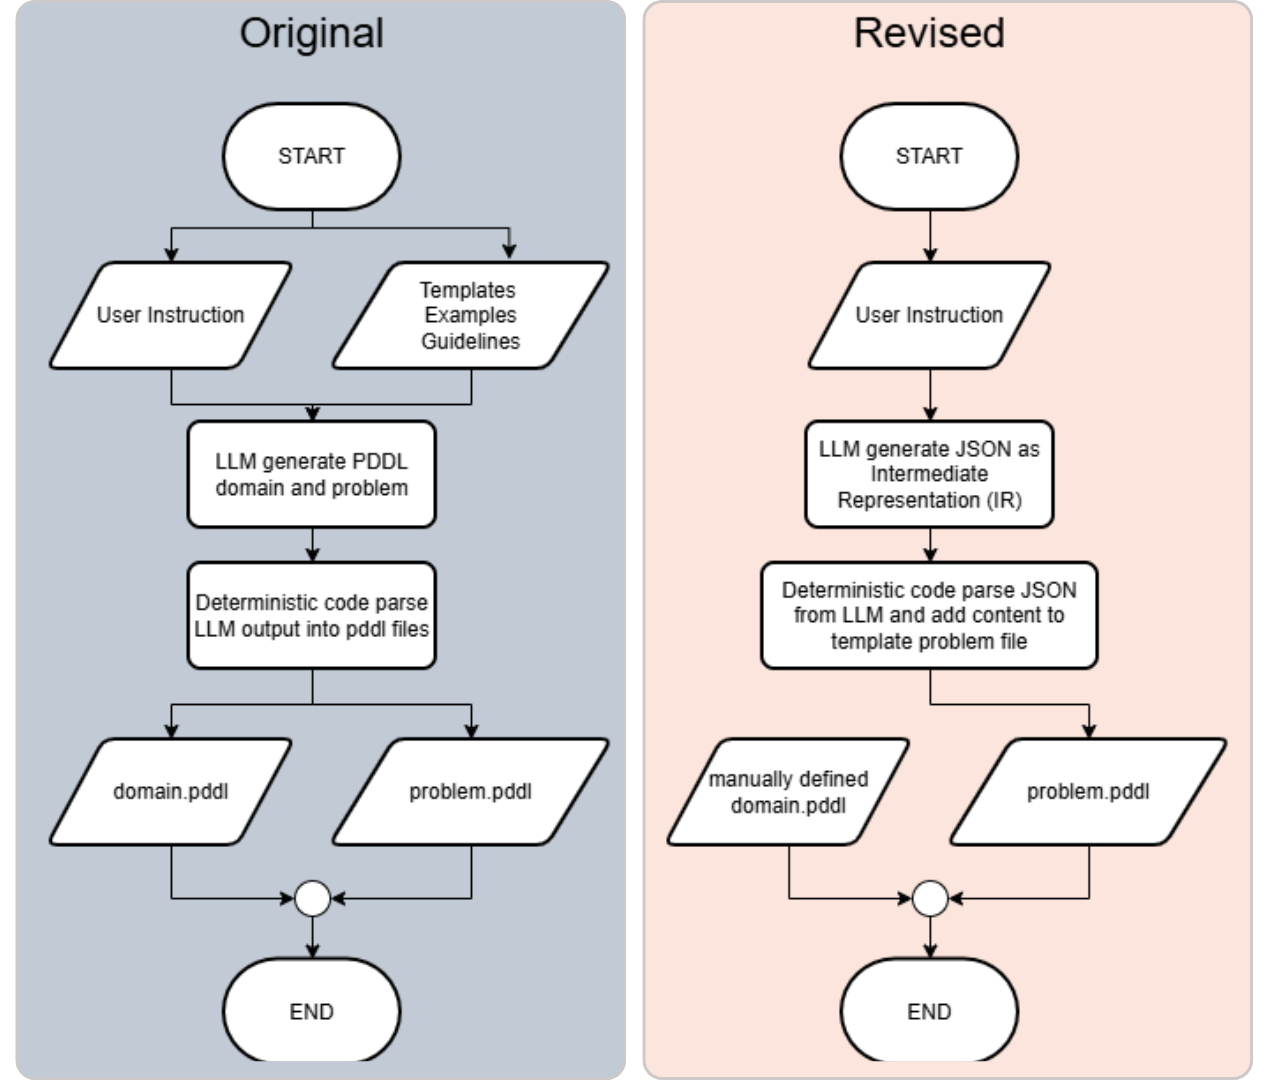
\includegraphics[width=\linewidth]{images/pddl_generation.png}
    \caption{Comparison of the original and revised automatic PDDL generation pipelines}
    \label{fig:pddl-pipeline}
\end{figure}

Preliminary evaluation indicates that this redesign significantly reduces syntax errors in generated planning problems, since the LLM is no longer responsible for producing raw PDDL code. The new pipeline also reduces both input and output token usage by removing large prompt templates and minimizing generated text. Furthermore, the intermediate JSON representation improves interpretability and debugging, as it provides a clear and structured description of the task before PDDL generation.

Overall, this approach increases reliability, efficiency, and system control while preserving the flexibility of natural language task specification.

\subsection{Hardware}

During system testing, we encountered an issue with the official UR ROS2 driver used to control the UR3e arm. After investigating the problem, we found that it corresponds to an open bug in the driver that affects the reliability of motion execution~\cite{ur-driver-issue}. Because the issue remains unresolved and the timeline for a fix is uncertain, relying solely on the driver poses a potential risk to the stability of the system.

To mitigate this risk, we implemented a backup control mechanism by developing an alternative implementation of the \texttt{low\_level\_planner\_executor} node that communicates with the robot using \textit{URScript}. URScript is the native scripting language of Universal Robots controllers, designed to directly command robot motion, gripper actions, and I/O operations through programmatic instructions executed by the robot controller~\cite{urscript-docs}.

Rather than relying on the ROS2 driver abstraction layer, this node sends URScript commands directly to the robot’s \textit{URControl} interface via TCP/IP socket communication. This approach follows the standard external control mechanism supported by Universal Robots and enables motion commands to be executed without the ROS2 driver middleware. The method is also consistent with techniques introduced in earlier coursework, where URScript programs are transmitted over a socket connection to the robot controller.

To maintain compatibility with the existing ROS2-side API, frame and orientation conversions were explicitly implemented within the \\\texttt{low\_level\_planner\_executor} node. This ensures that the same high-level Cartesian commands generated by the planner can still be executed correctly in the robot’s coordinate system, without requiring modifications to the ROS2 action interface or high-level planning components.

Let the ROS2-side Cartesian position be
\[
\mathbf{p}_R=\begin{bmatrix}x_R\\y_R\\z_R\end{bmatrix},
\]
and the URScript-side position be \(\mathbf{p}_U\).  
The ROS2 and UR frames are related by
\[
\mathbf{p}_U = \mathbf{T}\mathbf{p}_R,\qquad
\mathbf{T}=\mathrm{diag}(-1,-1,1)=\mathbf{R}_z(\pi).
\]
Hence
\[
(x_U,y_U,z_U)=(-x_R,-y_R,z_R).
\]

For orientation, ROS2 uses quaternions
\[
\mathbf{q}=(q_x,q_y,q_z,q_w),\qquad \|\mathbf{q}\|=1,
\]
while URScript uses rotation vector \(\mathbf{r}=(r_x,r_y,r_z)\), with
\[
\theta=\|\mathbf{r}\|,\quad \hat{\mathbf{u}}=\frac{\mathbf{r}}{\theta},\quad
\mathbf{q}=\left(\hat{\mathbf{u}}\sin\frac{\theta}{2},\cos\frac{\theta}{2}\right).
\]
Conversely, for quaternion-to-rotation-vector conversion:
\[
\theta=2\arccos(q_w),\quad
\mathbf{r}=
\begin{cases}
2(q_x,q_y,q_z), & \sqrt{1-q_w^2}<\varepsilon,\\[4pt]
\theta\frac{(q_x,q_y,q_z)}{\sqrt{1-q_w^2}}, & \text{otherwise}.
\end{cases}
\]

Frame conversion for absolute pose orientation is implemented via quaternion composition with a \(180^\circ\) rotation about \(z\):
\[
\mathbf{q}_T=(0,0,1,0),\qquad
\mathbf{q}_U=\mathbf{q}_T\otimes \mathbf{q}_R,
\]
where \(\otimes\) denotes quaternion multiplication. Since \(\mathbf{q}_T^{-1}=\mathbf{q}_T\), the same transform maps in both directions (self-inverse frame map).

For relative Cartesian commands \((\Delta x,\Delta y,\Delta z,\Delta\phi,\Delta\theta,\Delta\psi)\), the implemented mapping is
\[
(\Delta x_U,\Delta y_U,\Delta z_U)=(-\Delta x_R,-\Delta y_R,\Delta z_R),
\]
\[
(\Delta\phi_U,\Delta\theta_U,\Delta\psi_U)=(\Delta\phi_R,\Delta\theta_R,-\Delta\psi_R),
\]
then composed as
\[
\mathbf{q}_{k+1}=\mathrm{normalize}\!\left(\mathbf{q}_k\otimes
\mathbf{q}_{\Delta}(\Delta\phi_U,\Delta\theta_U,\Delta\psi_U)\right).
\]

This mathematical treatment ensures that direct URScript execution is kinematically consistent with the original ROS2-side API while removing dependence on the ROS2 driver middleware for runtime motion execution.

\vspace{0.5cm}

In addition to the control system modifications, several hardware improvements were implemented to enhance system robustness and repeatability.

First, the camera mounting setup was mechanically integrated with the base of the UR3e manipulator. The camera stand was rigidly fixed and secured in place to eliminate any relative movement between the camera and the robot base. By establishing a fixed and repeatable spatial relationship, this design removes the need for repeated extrinsic calibration before each operation. As a result, the transformation between the camera frame and the robot base frame remains constant across sessions, improving both system reliability and deployment efficiency.

Furthermore, a custom cable management solution was developed using additive manufacturing. A 3D-printed component was designed and fabricated to securely hold and guide the robot and camera cables along the structure. This component minimizes cable movement during operation, reducing the risk of entanglement, signal interruption, or mechanical interference with the robot’s motion. As shown in Fig.~\ref{fig:camera_mount}

The integration of these hardware modifications contributes to a more stable and user-friendly system, ensuring consistent sensing and execution performance while reducing setup time and operational errors.

\begin{figure}[h]
    \centering
    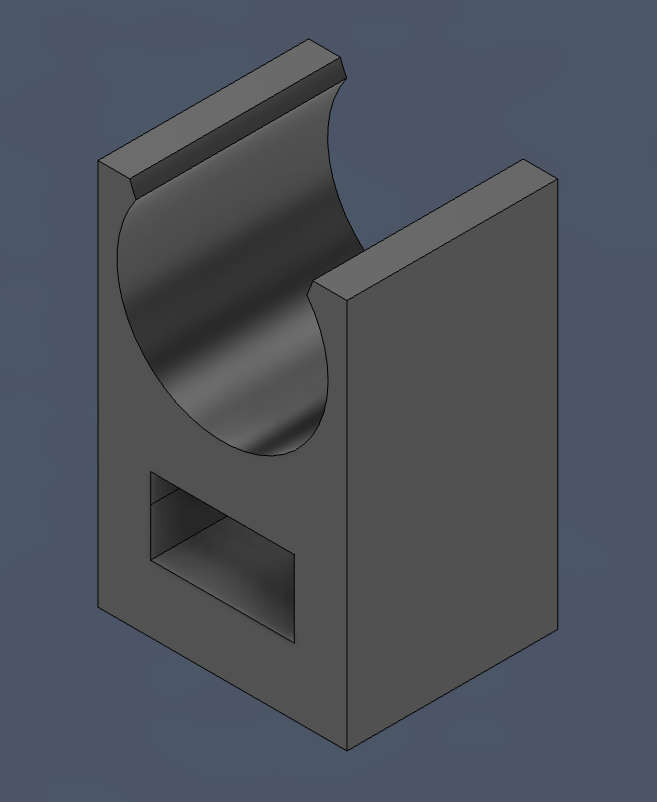
\includegraphics[width=0.6\linewidth]{images/cable mount.png}
    \caption{Custom cable mount integrated with the camera stand to secure and organize cables during operation.}
    \label{fig:camera_mount}
\end{figure}

\newpage
\section{Project Planning}
The project is structured around four primary technical area of concentration exluding any relevant paperwork tasks. These align seamlessly with the core enhancements, which will all be implemented in parallel: \textbf{image processing, speech processing, planning algorithms, and robotic arm integration}. The planned timeline is structured into weekly milestones to ensure iterative progress and early validation

\begin{figure}[htbp]
\centering
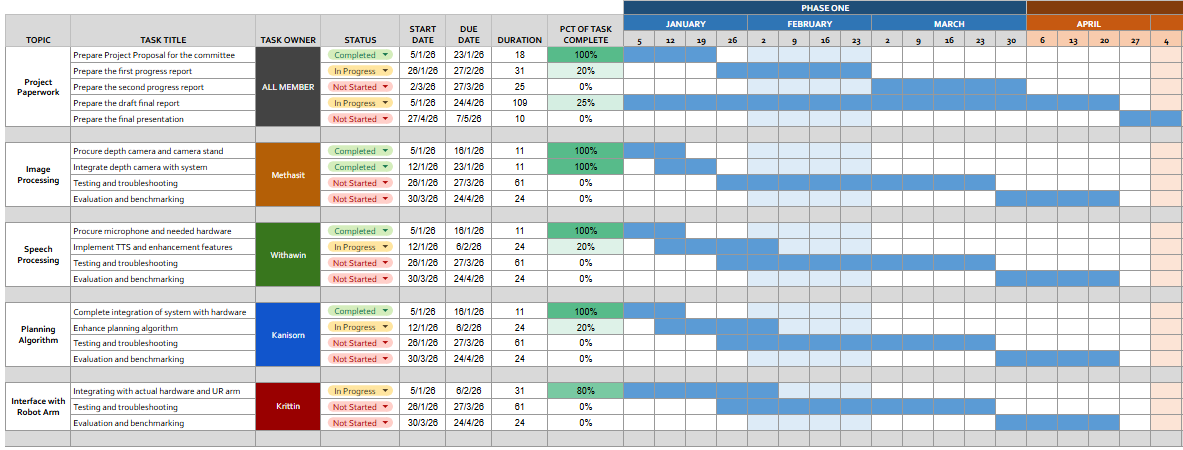
\includegraphics[width=\linewidth]{images/gantt_chart_sem_2.png}
\caption{A proposed project timeline scheduled for the project’s implementation in this semester}
\label{fig:gantt-chart}
\end{figure}

\subsection{Initial Timeline}

\subsubsection{Image Processing}
[2 Weeks] Procure depth camera and camera stand
\begin{itemize}
\item Identify suitable depth camera specifications based on workspace size, required accuracy, and compatibility with the existing system.
\item Procure and assemble the depth camera and adjustable camera stand for stable mounting.
\end{itemize}
[2 Weeks] Integrate depth camera with system
\begin{itemize}
\item Install and configure camera drivers and SDKs within the system environment.
\item Validate depth and RGB data acquisition and ensure reliable data streaming.
\end{itemize}
[9 Weeks] Testing and troubleshooting
\begin{itemize}
\item Develop and refine perception pipelines for object detection, localization, and pose estimation.
\item Perform iterative testing under varying lighting and workspace conditions to improve robustness.
\end{itemize}
[4 Weeks] Evaluation and benchmarking
\begin{itemize}
\item Quantitatively evaluate perception accuracy and latency.
\item Benchmark performance against task requirements for real-time robotic manipulation.
\end{itemize}

\subsubsection{Speech Processing}
[2 Weeks] Procure microphone and needed hardware
\begin{itemize}
\item Select and procure a microphone suitable for speech capture in a lab environment.
\item Verify hardware compatibility and audio input quality.
\end{itemize}
[4 Weeks] Implement TTS and enhancement features
\begin{itemize}
\item Implement text-to-speech pipeline for bidirectional interaction.
\item Apply noise reduction and audio preprocessing to improve recognition accuracy.
\end{itemize}
[9 Weeks] Testing and troubleshooting
\begin{itemize}
\item Test speech recognition across different speakers and command variations.
\item Improve error handling, command disambiguation, and response consistency.
\end{itemize}
[4 Weeks] Evaluation and benchmarking
\begin{itemize}
\item Measure command recognition accuracy and response latency.
\item Evaluate system usability in continuous human–robot interaction scenarios.
\end{itemize}

\subsubsection{Planning Algorithm}
[2 Weeks] Complete integration of system with hardware
\begin{itemize}
\item Establish communication interfaces between perception modules, planning modules, and hardware components.
\item Validate end-to-end data flow.
\end{itemize}
[4 Weeks] Enhance planning algorithm
\begin{itemize}
\item Extend and improve the planning framework.
\end{itemize}
[9 Weeks] Testing and troubleshooting
\begin{itemize}
\item Test the planner across diverse task scenarios and edge cases.
\item Refine decision-making logic to handle incomplete or uncertain inputs.
\end{itemize}
[4 Weeks] Evaluation and benchmarking
\begin{itemize}
\item Evaluate planning success rate, adaptability, and execution efficiency.
\item Benchmark planning performance in conjunction with perception and speech modules.
\end{itemize}

\subsubsection{Interface with Robot Arm}
[5 Weeks] Integrating with actual hardware and UR arm
\begin{itemize}
\item Improve interfaces for commanding the UR robotic arm.
\end{itemize}
[9 Weeks] Testing and troubleshooting
\begin{itemize}
\item Perform controlled physical experiments to ensure safe and reliable operation.
\end{itemize}
[4 Weeks] Evaluation and benchmarking
\begin{itemize}
\item Evaluate precision, repeatability, and task completion time.
\item Assess overall system performance in real-world tool-handling scenarios.
\end{itemize}

\subsection{Current Timeline}

\subsubsection{Image Processing}
The current progress is on schedule. Having transitioned from simulation to hardware, we refined our perception pipelines by implementing an Oriented Bounding Box (OBB) grasping strategy and a hybrid pixel-to-real-world calibration. We are currently benchmarking real-world accuracy and latency for real-time manipulation. With the foundational integration complete, our next focus is iterative testing to improve system robustness against environmental factors like varying lighting and dynamic workspace conditions.

\subsubsection{Speech Processing}

Both ASR and TTS components are on schedule and fully complete. The ASR node has been operational since semester 1, achieving a mean command recognition accuracy of 97.9\% across all participants. The TTS module has now been completed and integrated into the ROS2 system. The \texttt{tts\_topic\_node} subscribes to the \texttt{/tts} topic, synthesizes received text using the Coqui TTS VITS model, and plays the resulting audio in real-time through the system speakers via the ALSA utility \texttt{aplay}. The robot can now provide verbal feedback—confirming received commands and notifying the user upon task completion—closing the bidirectional interaction loop between the human operator and the robot.

\subsubsection{Planning Process}
The current progress is on schedule. Based on testing results, the automatic PDDL generation pipeline has been improved by introducing a structured intermediate representation (IR) instead of directly generating PDDL code. This change has reduced syntax errors, improved interpretability, and lowered token usage.

Future work will focus on further refining the system and benchmarking the planning pipeline across different task scenarios to evaluate robustness and efficiency.


\subsubsection{Interface with Robot Arm}

Progress is largely on schedule. The depth camera has been securely mounted at the base of the UR arm and is fully operational. Its spatial position relative to the UR base has been measured, and a consistent coordinate reference frame has been established to support camera-to-robot transformation. To further improve repeatability, the camera stand has been rigidly fixed to the robot base, eliminating relative displacement and removing the need for repeated calibration across sessions. The experimental workspace has also been prepared using a controlled visual background to improve perception reliability.

Mechanical integration has been further refined through the implementation of a structured cable management solution. A custom 3D-printed cable mount has been designed and installed on the camera stand to secure and guide the cabling. This prevents unwanted cable movement and ensures that wiring does not interfere with the UR arm’s range of motion. These improvements enhance system robustness, operational safety, and overall deployment efficiency.

\newpage
\section{Theory and Technical Backup}

\subsection{Voice Control Systems (VCS)}
Voice control systems have significantly transformed human-computer interaction by enabling users to interact with interfaces using voice commands and natural language. These systems leverage automatic speech recognition (ASR) to convert voice recordings into text, and advancements in deep learning have greatly enhanced their capabilities, alongside natural language processing. VCS offers numerous benefits, including saving users time and resources by providing quick services through an efficient interface without requiring extensive additional devices. They foster natural voice communication between users and devices, enhancing user comfort and creating a more intuitive interface. The adoption rate of voice-activated digital assistants has increased substantially, leading to a wide array of Internet of Things (IoT) devices incorporating voice-activated user interfaces for tasks ranging from creating grocery lists to controlling smart homes. Beyond smart gadgets and IoT, VCS technology is also applied in automotive systems to prevent accidents by allowing drivers to focus on their surroundings. VCS significantly improves the quality of life for various groups, including elderly people, children under four, and individuals with physical disabilities. They can provide complete control over home or office appliances, facilitate traffic regulation, and enhance healthcare systems~\cite{vcs}.

\subsection{Multimodal Automatic Speech Recognition}

\begin{figure}[htbp]
    \centering
    \includegraphics[width=0.8\linewidth]{asr}
    \caption{Multimodal ASR model architecture.
    (from~\cite{Chang2023})}
    \label{fig:asr}
\end{figure}

Multimodal Automatic Speech Recognition (ASR) enhances speech transcription by integrating visual context alongside audio signals, which is crucial for tasks such as embodied agents and human-robot interaction. By leveraging both modalities, multimodal ASR improves robustness and accuracy over traditional unimodal systems, achieving lower Word Error Rate (WER) and higher Recovery Rate (RR), especially under noisy or masked audio conditions. It is particularly effective at recovering visually salient words, such as object names, thereby increasing task completion rates in instruction-following scenarios~\cite{Chang2023},\cite{multi}.

Typical architectures combine a speech encoder, such as wav2vec 2.0, with a visual encoder, often based on CLIP-ViT, feeding both into a Transformer-based decoder that attends jointly to audio and visual features. Unlike unimodal ASR, which relies only on speech input, multimodal ASR grounds transcription in environmental context, reducing ambiguity and improving generalization to unseen speakers and settings~\cite{Chang2023},\cite{multi}.

Applications include benchmarks like ALFRED, where agents must interpret spoken instructions to navigate and manipulate objects, as well as real-world human-robot communication. Compared with unimodal baselines, multimodal ASR achieves superior masked word recovery (up to 30\% more) and mitigates performance degradation in noisy conditions~\cite{Chang2023},\cite{multi}. Challenges remain regarding generalization to real-world environments, as many studies rely on synthetic data and simplified noise models.

\subsection{Neuro-Symbolic Artificial Intelligence (NSAI)}

\begin{figure}[htbp]
    \centering
    \includegraphics[width=0.8\linewidth]{nsai-types}
    \caption{Neuro-Symbolic AI types
    (from~\cite{nsai})}
    \label{fig:nsai-types}
\end{figure}

Neuro-Symbolic Artificial Intelligence (NSAI) is an emerging paradigm that combines the strengths of neural networks with symbolic reasoning. Neural networks excel in pattern recognition and data-driven learning but often lack explainability and explicit reasoning capabilities, operating as "black boxes". In contrast, symbolic AI is inherently interpretable and excels in logical reasoning but struggles with perception from raw data and requires extensive manual knowledge engineering. NSAI aims to bridge these gaps by integrating the robust statistical learning of neural networks with the structured knowledge and logic of symbolic AI, enabling systems to reason, make decisions, and generalize knowledge more effectively from large datasets. This hybrid approach enhances interpretability, robustness, and trustworthiness, while also facilitating learning from less data~\cite{nsai}.\\
NSAI systems can be categorized into various architectures based on the connection between their neural and symbolic components, as shown in Figure~\ref{fig:nsai-types}. These include:
\begin{itemize}

    \item \textbf{Symbolic Wrapper (Type 1)}: Symbolic systems guide both input and output, leveraging neural networks internally for data-driven learning (e.g., DeepProbLog, Neuro-Symbolic Concept Learner (NSCL), hybrid neuro-symbolic robotics).

    \item \textbf{Symbolic [Neuro] (Type 2)}: Symbolic systems dominate, with neural modules used internally for perception and pattern recognition (e.g., in autonomous communication or scene interpretation).

    \item \textbf{Bidirectional Interaction (Type 3)}: Neural and symbolic components tightly interact, with neural models adjusting outputs based on symbolic constraints and symbolic modules evolving reasoning based on neural feedback (e.g., AlphaGo, AlphaZero, in robotics).

    \item \textbf{Sequential Connection (Type 4)}: Neural networks connect sequentially to symbolic systems via an explicit mapping layer, converting continuous neural outputs into structured symbolic knowledge (e.g., Neural Symbolic Machines (NSM)).

    \item \textbf{Embedded Symbolic Information (Type 5)}: Symbolic information is directly embedded into tensor representations, enhancing neural network reasoning in a differentiable manner (e.g., Logic Tensor Networks (LTNs)).

    \item \textbf{Deeply Integrated (Type 6)}: Symbolic structures are directly processed by neural networks, blending symbolic reasoning and neural computation seamlessly (e.g., Neural Theorem Provers (NTP), Graph Neural Networks (GNNs)).
\end{itemize}

\subsection{Large Language Model (LLM)}

\begin{figure}[htbp]
    \centering
    \includegraphics[width=0.5\linewidth]{transformer}
    \caption{The Transformer-model architecture
    (from~\cite{attention-is-all-you-need})}
    \label{fig:transformer}
\end{figure}

Large Language Models (LLMs), such as BERT and GPT-5, are pretrained neural networks that serve as powerful foundation models for language understanding and generation. They build on the Transformer architecture, shown in Figure~\ref{fig:transformer}, a sequence model that relies entirely on attention mechanisms and avoids recurrence or convolutions. The Transformer employs an encoder-decoder structure with stacked layers of multi-head self-attention and feed-forward networks, enabling the model to relate different positions within a sequence and capture diverse representation subspaces. Positional encodings are added to input embeddings to provide information about token order~\cite{attention-is-all-you-need}. LLMs represent words as vectors and acquire robust language and world knowledge through large-scale self-supervised learning, such as predicting masked words or the next word in a sequence. These models excel at tasks including machine translation, question answering, text classification, and text generation, leveraging vast amounts of text data to learn meanings and factual knowledge. Despite their capabilities, LLMs have limitations in deep understanding, reasoning, and completeness of knowledge, and raise societal concerns regarding bias and centralized model control~\cite{human-language-understanding}.

The reason why it is preferred over traditional Natural Language Processing (NLP) models is due to
the impressive ability to grasp broad contexts with little to no training. Mostly outperforms various
Natural Language Processing (NLP) techniques without having to fine-tune with execution cost.
Among the algorithms capable of handling a range of Natural Language Processing tasks, Large
Language Model (LLM) has not only frequently appeared in numerous past studies but has also
showcased immense potential for generating plans, transforming an initial world state into a desired state~\cite{plangenllm}.

\subsection{LangChain}

The open-source framework LangChain is designed to simplify the construction of applications powered by large language models (LLMs). In essence, LangChain supplies modular components, standardised abstractions, and orchestration utilities so that developers can build end-to-end LLM-based pipelines, agents, chatbots, retrieval-augmented generation (RAG) systems and more~\cite{langchain-docs}.

\subsubsection*{Overall architecture}
At a high level, LangChain can be thought of as layering on top of LLM providers (OpenAI, Anthropic, Google, etc.), providing a standard model-interface, a message history abstraction, tool-invocation support, memory/RAG support, and agent orchestration. Its goals include:
\begin{itemize}
\item A “standard model interface” so that different model providers can be swapped without deeply rewriting code. 

\item Pre-built abstractions such as “chains”, “agents” and “tools” so the developer doesn’t start from scratch. 

\item Capacity for persistence, human-in-the-loop control, durable execution and streaming, in part via its underlying runtime platform (LangGraph) though for many basic usages developers need not explicitly interface with it. 
\end{itemize}

\subsubsection*{Core concepts}

\begin{figure}[htbp]
    \centering
    \includegraphics[width=0.5\linewidth]{images/langchain-agent.png}
    \caption{Langchain Agent (from~\cite{langchain-docs})}
    \label{fig:langchain-agent}
\end{figure}

\paragraph{Models}
Models correspond to LLMs (or chat models) that produce text (or chat) responses. LangChain exposes a standard model interface so that developers can change the underlying provider (e.g., switching from OpenAI to Anthropic) without rewriting large parts of code. 

\paragraph{Messages}
Messages in LangChain represent the conversational context and follow roles like “system”, “user”, “assistant”. The message history can be passed to a model invocation so that it is aware of prior exchanges. This abstraction enables chat-style interactions and helps maintain context.

\paragraph{Tools}
Tools are external functions or actions that an agent can invoke. They might include retrieval of information, database queries, web APIs, or custom business logic. By combining the model’s generative power and tool invocation, agents built with LangChain can go beyond simple completion tasks into action-oriented workflows.

\paragraph{Short-Term Memory (and longer-term memory) }
Memory abstractions allow an agent to keep track of prior information and recall it during the interaction. Short-term memory might simply buffer recent messages; longer-term memory or retrieval-augmented memory might use vector stores or knowledge bases to fetch relevant prior context. This capability is critical for multi-turn dialogues or when the system must reference earlier interactions.

\paragraph{Agents}
Agents are orchestrators combining models, tools, messages, and memory into behaviour-enabled entities. A LangChain agent uses the model as the reasoning engine, deciding whether to call a tool (and which one), how to interpret responses, and iteratively work towards solution, as shown in Figure~\ref{fig:langchain-agent}. 

\subsection{Vision Language Model (VLM)}
\begin{figure}[htbp]
    \centering
    \includegraphics[width=0.8\linewidth]{images/vlm-structure.png}
    \caption{Structure of a Typical Vision Language Model (from~\cite{huggingface_vlms_2024})}
    \label{fig:vlm-structure}
\end{figure}

Vision Language Models (VLMs) are multimodal generative AI models that combine image and text understanding to perform a wide range of tasks, including visual question answering, image captioning, document analysis, and instruction-based image recognition. Many VLMs can also reason about spatial relationships in images, producing outputs like bounding boxes or segmentation masks. Architecturally, they usually consist of an image encoder, a projection layer that aligns image and text embeddings, and a text decoder for generating output, as shown in Figure~\ref{fig:vlm-structure}. Popular open-source VLMs include LLaVA, KOSMOS-2, Qwen-VL, CogVLM, and Fuyu-8B, each varying in model size, supported features such as chat or grounding, and image resolution~\cite{huggingface_vlms_2024}.

VLMs are powerful in zero-shot generalization, allowing them to handle unseen images and prompts without additional training. Furthermore, fine-tuning allows adaptation to specialized applications, such as educational tools, interactive assistants, or automated document evaluation. Their limitations include susceptibility to hallucinations, biases from training data, and high computational requirements for end-to-end training or large models~\cite{huggingface_vlms_2024}.
\subsection{Vision-Language-Action (VLA) Models}

\begin{figure}[htbp]
    \centering
    \includegraphics[width=0.8\linewidth]{images/vla.png}
    \caption{End-to-end Tokenization and Representation Process in VLA Models (from~\cite{vla})}
    \label{fig:vla}
\end{figure}

\begin{figure}[h]
    \centering
    \includegraphics[width=\linewidth]{images/vla-in-robot.png}
    \caption{Comparison between Monolithic and Hierarchical models (from~\cite{vla-in-robot})}
    \label{fig:vla-in-robot}
\end{figure}

Vision-Language-Action (VLA) models are multimodal AI systems that unify visual perception, natural language understanding, and embodied action into a single framework. Originally developed to overcome the fragmentation of traditional robotic pipelines, VLAs integrate pretrained Vision-Language Model (VLM) backbones with action policies, enabling robots to interpret high-level human instructions, reason about spatial relationships, and execute manipulation tasks in dynamic, real-world environments~\cite{vla}. For example, a VLA can follow commands such as “place the red mug next to the laptop onto the top shelf” by grounding visual perception, spatial reasoning, and motor control in a shared computational space. Architecturally, VLAs often rely on transformer-based models that fuse visual, linguistic, and state inputs into a common embedding~\cite{vla},\cite{vla-in-robot}.

A core innovation of VLAs lies in treating robot control as a sequence generation problem. Continuous actions, such as joint angles or end-effector poses, are discretized into tokens, allowing the model to autoregressively predict action tokens in the same way language models generate text. Alongside these, prefix tokens encode context from images and text, while state tokens represent the robot’s internal configuration, as shown in Figure~\ref{fig:vla}. This unified tokenization framework enables reasoning and execution to occur in the same latent space, with a de-tokenizer translating action tokens back into executable motor commands~\cite{vla},\cite{vla-in-robot}.

Two main architectural paradigms have emerged in robotic manipulation, as show in Figure~\ref{fig:vla-in-robot}. Monolithic models directly map multimodal inputs to low-level actions, sometimes combining a “slower” VLM for reasoning with a “faster” policy module for reactive control. In contrast, hierarchical models decouple high-level planning from low-level execution, with a planner producing intermediate representations (e.g., subtasks or keypoints) for downstream policies~\cite{vla-in-robot}. These designs balance efficiency, interpretability, and modularity, depending on task complexity.

VLAs represent a shift from handcrafted pipelines toward end-to-end, language-driven policy generation. They leverage the semantic grounding of VLM pretraining while extending it to action, offering broad potential in robotics, embodied assistants, and human-robot interaction. However, they face limitations such as high computational requirements, difficulty in precisely grounding abstract instructions, and restricted generalization beyond training distributions~\cite{vla},\cite{vla-in-robot}.

\subsection{Planning Domain Definition Language (PDDL)}
\label{sec: pddl}
Planning Domain Definition Language (PDDL) is a standardized language for modeling automated planning problems in artificial intelligence. It separates a domain (the rules of the world: types, predicates, and actions) from a problem (a specific initial state and goal). PDDL allows users to specify objects, predicates, actions, and goals in a structured way, enabling automated planners to generate sequences of actions that achieve desired outcomes. However, PDDL is deliberately neutral: it encodes the physics of a domain without embedding heuristics or solving strategies, meaning many planners only support subsets of the language~\cite{pddl-1.2}.

A classic illustration is the Briefcase World. Here, moving the briefcase also moves everything inside it, while objects can be put in or taken out. Below, the domain defines actions and the problem specifies the goal of moving a dictionary and briefcase to the office while leaving a paycheck at home:

\begin{lstlisting}[language=PDDL]
(define (domain briefcase-world)
  (:requirements :strips :typing :conditional-effects)
  (:types location physob)
  (:constants B - physob)
  (:predicates (at ?x - physob ?l - location) (in ?x ?y - physob))
  (:action mov-b
    :parameters (?m ?l - location)
    :precondition (and (at B ?m) (not (= ?m ?l)))
    :effect (and (at B ?l) (not (at B ?m))
                 (forall (?z)
                   (when (and (in ?z) (not (= ?z B)))
                     (and (at ?z ?l) (not (at ?z ?m)))))))))
  (:action put-in
    :parameters (?x - physob ?l - location)
    :precondition (not (= ?x B))
    :effect (when (and (at ?x ?l) (at B ?l))
                  (in ?x)))
  (:action take-out
    :parameters (?x - physob)
    :precondition (not (= ?x B))
    :effect (not (in ?x)))
                     
(define (problem get-paid)
  (:domain briefcase-world)
  (:init (place home) (place office)
         (object p) (object d) (object b)
         (at B home) (at P home) (at D home) (in P))
  (:goal (and (at B office) (at D office) (at P home))))

\end{lstlisting}

PDDL has evolved from its early versions, like PDDL 1.2, which used predicate logic with true/false properties and actions, to more expressive forms. PDDL 2.1 introduced durative actions and numeric fluents for modeling time and resources, while PDDL 2.2 added derived predicates and timed literals. PDDL 3.0 incorporated soft constraints and preferences with costs, and PDDL+ enabled modeling of processes and uncontrollable events. Specialized variants such as PPDDL, NDDL, and MADDL were later developed for domain-specific planning needs~\cite{pddl}.

\subsection{Fast Downward}

\begin{figure}[htbp]
\centering
\includegraphics[width=\linewidth]{images/fast_downward_execution.png}
\caption{The three phases of Fast Downward’s execution (from~\cite{the-fast-downward-planning-system})}
\label{fig:fd_execution}
\end{figure}

The Fast Downward planning system is a domain-independent classical planner built for deterministic planning tasks encoded in PDDL~\cite{the-fast-downward-planning-system}. It employs a forward search strategy, but crucially it does not operate directly on the propositional PDDL as given; instead it transforms the input into a multi-valued planning task (MPT) representation, and then compiles further structural knowledge (causal graphs, domain‐transition graphs, etc.) to support heuristic search~\cite{the-fast-downward-planning-system}.

\bigskip

The Fast Downward planning system operates in three main phases, as illustrated in Figure~\ref{fig:fd_execution}:

\begin{itemize}
\item \textbf{Translation.} The input PDDL task (with propositional facts, operators, axioms) is first normalized, grounded, invariants are synthesized, and an equivalent multi‐valued planning task is generated. This step is designed to expose structure (e.g., mutual exclusion of propositions) that is otherwise implicit in the propositional encoding.
\item \textbf{Knowledge Compilation.} From the MPT representation the planner builds data structures such as domain‐transition graphs (for each variable, how its values can change under operators), the causal graph (showing dependencies between variables), successor‐generators (efficient enumeration of applicable operators), and axiom evaluators (to compute derived variable values).
\item \textbf{Search.} Given the compiled knowledge structures, the planner uses heuristic best‐first search variants. Its signature heuristic is the causal-graph heuristic, which uses the MPT and the causal graph to estimate goal distances by solving subproblems induced by individual variables (in a hierarchical manner). The planner also supports multi‐heuristic best‐first search (combining the causal‐graph heuristic with the FF heuristic) and a non-heuristic method called focused iterative‐broadening search. Preferred operators (analogous to helpful actions) and deferred heuristic evaluation further enhance search efficiency.
\end{itemize}

\bigskip

The planner is open‐source, publicly available via its website~\cite{fast-downward-website}. The typical workflow includes modeling the domain in PDDL, running Fast Downward to translate and compile, then searching for a plan. Many derivative planners and portfolios build on its infrastructure. For academic and practical evaluation tasks, the strong support for the MPT translation and causal heuristic make it particularly useful when one can afford the preprocessing overhead.

\subsection{ROS2}

\begin{figure}[htbp]
    \centering
    \includegraphics[width=\linewidth]{images/ros2_architecture.png}
    \caption{ROS2 conceptual architecture, illustrating nodes, topics, services, and actions.}
    \label{fig:ros2_architecture}
\end{figure}


ROS2 (Robot Operating System 2) is an open-source middleware framework designed to support the development of distributed, real-time robotic applications. Building upon the foundation of ROS1, ROS2 introduces improved communication paradigms, enhanced reliability, real-time capability, and cross-platform support, making it more suitable for both research and industrial deployment.

At its core, ROS2 is structured around nodes, which are independent processes that communicate through a decentralized publish/subscribe architecture. Nodes exchange messages over topics, invoke synchronous operations through services, and trigger asynchronous long-running tasks via actions. This modular design ensures scalability and flexibility for complex robotic systems. The underlying communication is handled through the Data Distribution Service (DDS), providing discovery, quality-of-service (QoS) policies, and secure data exchange between distributed components.

The ROS2 execution model is further supported by concepts such as parameters for runtime configuration, launch files for orchestrating multiple nodes, and lifecycle management for robust system control. Additionally, the framework introduces tools such as \texttt{ros2cli} for command-line interaction, \texttt{rclcpp}/\texttt{rclpy} for C++ and Python client libraries, and \texttt{rviz2} for visualization. Together, these components form an ecosystem that simplifies robotic software integration while maintaining performance and portability across platforms.

ROS2 represents a shift from experimental middleware to a production-ready robotics framework. Its modularity, DDS-based communication, and lifecycle-aware design provide strong technical backing for robotics research and application development, though challenges such as system complexity and tuning persist~\cite{ros2-doc}.

\subsection{MoveIt2}

MoveIt2 is a motion planning framework for ROS2 that integrates kinematics, collision checking, planning, and execution into a unified pipeline. It enables robots to interpret high-level goals, such as "pick the object and place it in the bin", and compute collision-free, dynamically feasible trajectories to accomplish them.

At its core, MoveIt2 is structured around modular components, as shown in Figure~\ref{fig:moveit_pipeline}. The Kinematics module translates between joint states and end-effector poses, while the Planning Scene Monitor maintains an up-to-date model of the environment. The Motion Planning system leverages planners such as OMPL or TrajOpt to generate valid paths, which are refined in the Trajectory Processing stage into smooth, executable trajectories.

The central move\_group node provides a user-facing API for motion planning and execution, while advanced features like Hybrid Planning combine long-horizon strategies with local reactive control. The MoveIt Task Constructor further extends this capability by composing multi-step task sequences, making it suitable for applications such as bin picking and assembly.

MoveIt2 shifts motion planning from isolated libraries toward a flexible, extensible middleware. Its modular design promotes reusability and adaptability across robotic domains, though challenges remain in accurate modeling, computational cost, and system tuning~\cite{moveit-doc},\cite{moveit2}.

\begin{figure}[htbp]
    \centering
    \includegraphics[width=\linewidth]{images/moveit_pipeline.png}
    \caption{MoveIt2 motion planning pipeline.}
    \label{fig:moveit_pipeline}
\end{figure}

\subsection{Gazebo}

Gazebo is an open-source robotics simulation platform that enables realistic, high-fidelity simulation of robots, sensors, and environments. It allows developers to test algorithms, design robots, and train AI models in a virtual setting before deploying on hardware.

Gazebo uses a modular architecture, separating physics, rendering, sensor simulation, and communication. The server handles physics and sensor updates, while the client provides visualization and user interaction. Robots and environments are described using the Simulation Description Format (SDF), and plugins extend functionality for custom behaviors and controllers.

Integrated with ROS, Gazebo allows seamless simulation-to-hardware transitions. Its strengths include realistic physics, sensor modeling, and extensibility through plugins, making it suitable for research, education, and development of both single and multi-robot systems~\cite{gazebo}


\subsection{Artificial Intelligence in Image Processing}

\begin{figure}[htbp]
    \centering
    \includegraphics[width=0.8\linewidth]{images/CNN.png}
    \caption{Convolutional Neural Network (CNN) Architecture for Image Classification}
    \label{fig:cnn}
\end{figure}

Artificial Intelligence (AI) has significantly transformed image processing, introducing cutting-edge methods and applications that streamline processes for enhanced speed and accuracy. Image processing itself involves understanding digital images as pixel-based visual information, along with various formats (e.g., JPEG, PNG), enhancement techniques (such as adjusting brightness or reducing noise), and filtering/restoration procedures. Within this framework, AI, especially through deep learning architectures like Convolutional Neural Networks (CNNs) and Generative Adversarial Networks (GANs), enables systems to extract crucial features, recognize objects, segment images, and even generate realistic visual content. This capability allows robots to interpret visual information similarly to humans, finding practical uses in areas like autonomous vehicles for navigation and surveillance systems for security~\cite{ai-in-image-processing}.

The capabilities of AI image processing are broad and impactful, including accuracy enhancements, efficiency improvements, and the capacity to manage large datasets. AI has demonstrated significant success in improving diagnostic accuracy and early disease detection in healthcare, optimizing industrial packing strategies for greater efficiency and reduced waste, and enabling real-time applications and deployment on devices with limited resources through crucial optimization techniques like model compression. Advanced functions such as object detection, image segmentation, and content-based image retrieval are also facilitated by these methods. Despite these advantages, the application of AI in image processing faces notable limitations and ethical challenges. These include critical concerns regarding data privacy, interpretability of AI decisions, and the potential for biases embedded in training data to produce prejudiced results. Therefore, ensuring responsible, transparent AI systems that respect cultural diversity and address potential impacts on employment are vital for the technology's continued development~\cite{ai-in-image-processing}.

\subsection{Universal Robots Arm (UR ARM)}

\begin{figure}[htbp]
    \centering
    \includegraphics[width=0.8\linewidth]{images/UR_Arm_pic.png}
    \caption{the Move Screen interface of a Universal Robots (UR) robotic arm's ~\cite{urarm}}
    \label{fig:urarm}
\end{figure}

The Universal Robots (UR) robotic arm is a widely adopted collaborative robotic manipulator (cobot) designed for flexible deployment in industrial, engineering, and research settings. Unlike traditional industrial robots, UR arms are specifically engineered to operate safely alongside humans without requiring extensive physical barriers, thanks to their integrated safety features, lightweight design, and force-limiting mechanisms. These properties make UR arms particularly suitable for human-robot collaboration in dynamic environments such as manufacturing, assembly, and tool-handling applications.
From a technical perspective, UR arms employ high-precision servo motors and torque sensors at each joint, enabling six degrees of freedom for dexterous manipulation tasks. Their kinematic flexibility allows execution of both structured and unstructured manipulation tasks, such as grasping, tool usage, and assembly operations. Additionally, UR arms are equipped with programmable interfaces, including graphical user interfaces (GUI), teach pendants, and increasingly, APIs compatible with external AI systems~\cite{urarm}. This enables integration with higher-level control architectures, such as neuro-symbolic AI (NSAI) or large language models (LLMs), for advanced planning, reasoning, and adaptive execution.

\subsection{URScript}

URScript is the native scripting language developed by Universal Robots for programming and controlling their collaborative robotic arms. It provides a textual programming interface that allows users to control robot motion, interact with sensors and I/O devices, and integrate the robot with external software systems. In the Universal Robots ecosystem, programs created through the graphical programming interface \textit{PolyScope} are internally translated into URScript commands, which are then executed by the robot controller~\cite{urscript-docs}. Consequently, URScript represents the fundamental low-level interface used by the controller to perform robot operations.

\subsubsection*{Overall architecture}

Universal Robots systems can be controlled at two main levels: the graphical user interface level through PolyScope, and the script level through URScript~\cite{urscript-manual}. At the script level, programs are written as text-based instructions that are interpreted by the robot controller (URControl). URControl runs as a service on the robot's control computer and executes commands sent either from PolyScope or from an external client over a TCP/IP connection.

URScript programs can therefore be executed in multiple ways:
\begin{itemize}
\item Directly within PolyScope using script nodes embedded in a graphical program.
\item As standalone script files executed by the robot controller.
\item Remotely from external computers by sending URScript commands over a network socket to the robot controller.
\end{itemize}

This architecture allows URScript to serve both as a low-level control interface and as an integration mechanism for external software frameworks such as ROS or custom control applications.

\subsubsection*{Core language features}

URScript is designed as a high-level scripting language with a syntax similar to Python, making it relatively easy to learn for users familiar with modern programming languages. The language includes common programming constructs such as variables, functions, and control-flow statements, enabling developers to implement complex robotic behaviours.

\paragraph{Variables and data types}
URScript supports several basic data types including integers, floating-point numbers, booleans, lists, and poses. Pose data types are particularly important in robotics applications, as they represent the position and orientation of the robot's tool center point (TCP) in Cartesian space.

\paragraph{Control structures}
The language provides standard control-flow constructs such as \texttt{if} statements, loops, and function definitions. These constructs allow users to create structured programs and reusable subroutines that organize complex robot behaviours.

\paragraph{Motion commands}
A key feature of URScript is its built-in motion control functions. Commands such as \texttt{movej}, \texttt{movel}, and \texttt{movep} allow the robot to move between poses using joint-space, linear, or process-oriented trajectories. These commands typically include parameters for velocity, acceleration, and blending radius, enabling precise control of robot motion.

\paragraph{I/O and sensor interaction}
URScript also provides functions for interacting with the robot's digital and analog I/O interfaces. These functions allow the program to read sensor signals, control external devices such as grippers or conveyors, and synchronize robot actions with other equipment in an automated system.

\paragraph{External communication}
Another important capability of URScript is communication with external systems through network protocols such as TCP/IP sockets or industrial communication standards like Modbus TCP. This functionality enables integration with higher-level control software, PLCs, and robotic frameworks.

Overall, URScript provides a flexible and powerful mechanism for controlling Universal Robots manipulators, enabling both simple task programming and advanced integration with external robotic software systems. In many applications, URScript is used as the underlying execution layer for commands generated by higher-level frameworks such as ROS-based drivers or custom control software.


\newpage
\section{Project Outcome}

By the deadline of this project , there will be a detailed report documenting how the proposed AI robot arm planning approach performs on the TASK and Motion Planning (TAMP) benchmarks, compared to other baseline solutions. This report will highlight the assistant's strength in combining voice-command understanding, image-processing, and robotic manipulation for engineering tool-handling task.

Accompanying the project is a robotic prototype built on a UR5e robotic arm equipped with a parallel gripper. The robot is connected to a workstation running for UR Arm Library, which serves as the central processing unit, integrating both perception and planning modules. Through this workstation, the robot interfaces with:

\begin{itemize}
    \item \textbf{Camera}:A depth camera for real-time object recognition and workspace mapping.
    \item \textbf{Microphone}: A input with ASR(Automatic Speech Recognition) pipeline for natural voice-command input.
    \item \textbf{Robotics}: Motion controllers for safe execution of grasping and tool-passing tasks. 
\end{itemize}

With these specifications, the prototype is expected to demonstrate the following core capabilities:

\subsection{Autonomous Planning:}

The robot should be able to decompose natural voice instructions (e.g., “pass me the wrench, then place the screwdriver on the table”) into a symbolic task plan and execute it.

\subsubsection{Path and Motion Safety}
The robot should plan trajectories that are collision-free, navigating cluttered tool-workspaces without endangering users or damaging objects.

\subsubsection{Generalization:} The assistant should adapt to unseen scenarios, such as handling tools of unfamiliar shapes or working in rearranged environments, while maintaining performance targets of more than 70 \% sequence correctness and 85 \% collision-free trajectories in simulation when executing TAMP tasks~\cite{tamp}

\subsubsection{Human Collaboration:} The robot must safely pass tools to human collaborators by respecting dynamic human safety zones, pausing or re-planning if a human unexpectedly enters its workspace.

Overall, at the surface level, the outcome of this project will be a robot arm assistant capable of autonomously planning and executing tool-handling tasks in engineering workshop scenarios. On a deeper level, this project demonstrates how combining neural and symbolic AI can produce robots that reason about complex tasks, adapt to novel environments, and safely interact with humans. In the long run, this prototype serves as a foundation for intelligent robotic assistants in manufacturing, laboratories, and educational workshops, showing how autonomous planning can be extended from research into real-world engineering applications.

\newpage
\section{Summary and Benefit to Real Industry}

This project aims to build a prototype of a robotic planning assistant that integrates Large Language Models (LLMs) with symbolic reasoning for tool-handling in engineering environments. The LLM is responsible for translating natural language instructions into multi-step task plans, while Symbolic AI serves as a verification layer, checking for correctness and preventing unsafe or hallucinated actions. The prototype will serve as a proof of concept for how hybrid planning architectures can enable safe, interpretable, and adaptable robotic assistants in industrial settings.

As noted in recent studies~\cite{enhancing-interpret},\cite{learning-neuro-symbolic},\cite{code-as-symbolic-planner},\cite{code-as-policies}, LLMs have demonstrated strong capabilities in task decomposition, code generation, and multimodal integration, while symbolic systems contribute precision, interpretability, and logical consistency ~\cite{code-as-symbolic-planner}. Combining these approaches enhances reliability and operator trust, allowing robots to adapt to unseen scenarios while remaining verifiable.

The expected outcome is a system that reduces downtime, improves safety, and supports human-robot collaboration by enabling robots to be re-tasked directly from natural language instructions without extensive retraining. If successful, this approach can extend beyond tool-handling to applications in \textbf{manufacturing, construction, healthcare, and hazardous environments}, offering a scalable framework for safe and efficient robotic deployment across industries.

\newpage
\section{Roles and Responsibilities}

{
\renewcommand{\arraystretch}{1.3} % 1.3x default row height
\begin{table}[h!]
    \centering
    \begin{tabular}{|l|p{6cm}|l|}
        \hline
        \textbf{Project Task} & \textbf{Task Description} & \textbf{Assigned to} \\
        \hline
        Planning Algorithm & Design and implement a task planning framework that translates perception and speech inputs into executable robotic actions, with emphasis on symbolic reasoning and system integration & Kanisorn Sangchai \\
        \hline
        Image Processing & Integrate a depth camera and develop perception pipelines for object detection, localization, and pose estimation, followed by testing and performance evaluation & Methasit Boonpun \\
        \hline
        Speech Processing & Implement speech-to-text and text-to-speech modules for command-based interaction, including noise handling, command parsing, and system-level integration & Withawin Kraipetchara \\
        \hline
        Interface with Robot Arm & Develop interfaces for controlling the UR robotic arm, validate motion execution through simulation, and perform safe real-world integration and testing & Krittin Kitjaruwannakul \\
        \hline
        Project Paperwork & Prepare the project proposal, progress documentation, final report, and presentation materials & All Members \\
        \hline
    \end{tabular}
    \caption{An outline of major responsibilities assigned to each member within the project}
    \label{tab:roles_responsibilities}
\end{table}
}

The roles and duties of this project revolve around the four main features. Each feature is allocated to a team member as outlined in Table~\ref{tab:roles_responsibilities}

\newpage
\section{Results}

\subsection{Vision}

Vision pipeline was evaluated in simulation using Gazebo across 5 distinct worlds, each containing 5 objects. The evaluation focused on object detection, classification, grasp pose estimation, and scene understanding, as well as the accuracy of pixel-to-real-world coordinate conversion. The testing procedure for each module is as follows:

\begin{itemize}
    \item \textbf{SAM (Segment Anything Model)}: Each object in the world was segmented, and results were recorded in terms of bounding box coordinates, detection confidence, and Average Precision (AP) for IoU $\geq 0.5$.
    
    \item \textbf{CLIP Classifier}: Detected object regions were classified using the CLIP model. Performance metrics included predicted labels, confidence scores, and Top-1 accuracy for each object.
    
    \item \textbf{GraspNet}: For each detected object, the system estimated grasp poses. Recorded metrics included position $(x, y, z)$, orientation $(x, y, z, w)$, quality score $Q$, grasp width, approach angle, and overall success rate (SR) in simulation grasps.
    
    \item \textbf{Scene Understanding}: The module evaluated object relations and spatial context. Metrics recorded included the predicted relation list, spatial accuracy, and adjacency accuracy between objects.
    
    \item \textbf{Pixel-to-Real Conversion}: Depth and RGB data were used to convert pixel coordinates to real-world coordinates. Accuracy was measured using Root Mean Square Error (RMSE) against ground-truth positions in Gazebo.
\end{itemize}

\paragraph{Evaluation Procedure}
For each world:
\begin{enumerate}
    \item Spawn 5 objects with randomized positions and orientations.
    \item Run the \texttt{/vision/run\_pipeline} service once to process the entire scene.
    \item Collect output from each module (SAM, CLIP, GraspNet, Scene Understanding) and log metrics.
    \item Compare pixel-to-real coordinates against ground truth for RMSE computation.
    \item Repeat for all 10 worlds to obtain aggregate performance statistics.
\end{enumerate}

\subsubsection{Experimentation and Evaluation}

\begin{table}[h!]
\centering
\caption{Summary of vision-module benchmark results (5 worlds $\times$ 5 objects = 25 objects)}
\label{tab:vision-eval}
\begin{tabular}{lcc}
\hline
\textbf{Model} & \textbf{Benchmark (metric)} & \textbf{Result} \\
\hline
SAM (segmenter) & AP (IoU $\ge$ 0.5) & $0.7408$ \\
CLIP (region classifier) & Top-1 Accuracy (TOP1 / ALL) & $0.85$ \\
GraspNet (grasp proposal) & Quality Score (Q) & $0.746$ \\
Scene understanding & Spatial Accuracy (Corrected Relation/ Total) & $0.98$ \\
Pixel-to-Real Service & RMSE (meters) & $0.05365$ \\
\hline
\end{tabular}
\end{table}

The vision pipeline was evaluated on five distinct Gazebo worlds, each populated with five unique objects (25 object instances total). For each object we ran the perception stack end-to-end (SAM $\rightarrow$ CLIP $\rightarrow$ GraspNet $\rightarrow$ Scene module) and aggregated per-object scores into the single summary shown in Table~\ref{tab:vision-eval}. Below we explain each metric, how it was computed, and why it was chosen.

\paragraph{SAM — Average Precision (AP) at IoU $\ge$ 0.5.}
We report region-level Average Precision computed using a single IoU threshold of 0.5 (the PASCAL VOC–style AP@0.5 convention). For each predicted mask we compute the Intersection-over-Union (IoU) with the ground-truth mask:
\[
\mathrm{IoU} = \frac{|\text{Prediction} \cap \text{GroundTruth}|}{|\text{Prediction} \cup \text{GroundTruth}|}.
\]
A prediction is considered a true positive when IoU $\ge 0.5$; precision–recall curves are constructed across confidence thresholds and AP is the area under the precision–recall curve for the instance class. The reported $0.7408$ is the mean AP over all 25 object instances. This AP formulation follows established segmentation/detection protocols and is consistent with how promptable segmentation models (e.g., SAM) are typically evaluated. \cite{kirillov2023segment,padilla2021metrics}

\paragraph{CLIP — Top-1 Accuracy.}
CLIP is used to assign a semantic label (region caption/class) to each SAM proposal. We evaluate classification accuracy in the standard Top-1 sense: the model's highest-scoring label is compared to the ground-truth label; Top-1 accuracy is the fraction of proposals for which this highest score equals the ground truth. The reported value ($0.85$) is computed as
\[
\text{Top-1 Acc.} = \frac{\#\{\text{correct top predictions}\}}{\#\{\text{evaluated proposals}\}}
\]
over the 25 objects. Using CLIP for region classification leverages its zero-shot image–text embedding ability and this metric directly measures semantic assignment fidelity. \cite{radford2021clip,openai_clip}

\paragraph{GraspNet — Quality Score (Q).}
For grasping we used GraspNet-style grasp proposals and evaluated a per-proposal \emph{Quality Score} (Q). In practice Q is a consolidated score that reflects the predicted grasp's feasibility under geometric and collision constraints (for example: antipodal/force-closure geometry, clearance from collisions, and stability heuristics used in the dataset/simulator). During evaluation we rank proposals by their Q value and compute the average Q over the top-K proposals per object (K chosen to match the GraspNet evaluation protocol used in our simulator). The reported aggregate score $0.746$ is the mean Q across 25 objects. This metric correlates with practical grasp success probability when proposals are executed in simulator/hardware and follows the GraspNet benchmarking philosophy. \cite{fang2020graspnet,wu2024grasping}

\paragraph{Scene understanding — Spatial Accuracy.}
Spatial Accuracy measures how often the scene module correctly predicts metric spatial relationships (e.g., object coordinates relative to a world origin, and pairwise spatial predicates such as \texttt{left-of}, \texttt{on-top-of} within the chosen tolerance). Concretely, we evaluate:
\begin{itemize}
  \item \textbf{Positional error}: Euclidean distance between predicted object centroid and ground-truth centroid in world coordinates; a prediction is \emph{spatially correct} when the error $\leq$ a task threshold (here, 2\,cm).
  \item \textbf{Relational correctness}: fraction of pairwise relation queries (e.g., ``is A left of B'') answered correctly.
\end{itemize}
Spatial Accuracy reported ($0.98$) is the fraction of all positional + relation checks that passed. This combined metric matches recent 3D spatial understanding benchmarks which evaluate both metric and relational components. \cite{daxberger2025mmspatial,zhao2023vsd}


\paragraph{Pixel-to-Real Service — RMSE (Root Mean Square Error).}
The Pixel-to-Real module converts 2D pixel coordinates and depth values into 3D world coordinates using the camera intrinsic model. We evaluate accuracy using RMSE between predicted world points $\hat{p}_i$ and ground-truth world points $p_i$:
\[
\mathrm{RMSE} = 
\sqrt{
\frac{1}{N} \sum_{i=1}^{N} 
\left\| \hat{p}_i - p_i \right\|^{2}
}.
\]
This metric is widely used for depth-based 3D reconstruction and camera geometry evaluation. \cite{yin2021learning,teed2020raft3d}  
Our Pixel-to-Real service achieves an RMSE of \textbf{0.05365\,m}, demonstrating high accuracy in metric projection and depth-to-world mapping across all worlds.


\subsection{Speech}

The speech module encompasses two components: Automatic Speech Recognition (ASR) for receiving voice commands, and Text-to-Speech (TTS) for providing spoken feedback. Both have been implemented, evaluated, and fully integrated into the ROS2 system.

\subsubsection{Automatic Speech Recognition}

The ASR system has been fully integrated as a ROS2 node, providing real-time speech-to-text functionality, deactivation word recognition, and an emergency stop mechanism. The node continuously captures live audio streams, transcribes commands in real time, and publishes recognized sentences to the planning node only if the sentence ends with the deactivation word ``execute.'' The emergency stop allows immediate halting of robot motion with the command ``STOP'' and can be deactivated using the word ``OKAY.'' This workflow ensures responsive, safe, and controlled interaction between the human operator and the robot.

\subsubsection{Experimentation and Evaluation}

The ASR system was evaluated using a set of 30 task commands of varying complexity. Three participants (Kanisorn, Methasit, and Withawin) each performed all tasks. System performance was measured in terms of successful recognition and correct transmission of the command to the planning node.

\begin{table}[H]
\centering
\small
\caption{ASR Command Recognition Success for Three Participants}
\resizebox{\textwidth}{!}{%
\begin{tabular}{lccc}
\hline
\textbf{Sentences/People} & \textbf{Kanisorn} & \textbf{Methasit} & \textbf{Withawin} \\
\hline
Pick up the red cube and place it on the table, execute. & 12/12 & 12/12 & 12/12 \\
Move the arm to the home position, execute. & 8/8 & 8/8 & 8/8 \\
Grab the green cylinder and put it in the bin, execute. & 11/11 & 11/11 & 11/11 \\
Rotate the wrist clockwise 90 degrees, execute. & 7/7 & 7/7 & 7/7 \\
Pick up the yellow object and stack it on the red cube, execute. & 13/13 & 13/13 & 13/13 \\
Extend the arm forward slowly, execute. & 6/6 & 6/6 & 6/6 \\
Move to the left side of the table, execute. & 9/9 & 9/9 & 9/9 \\
Stop. & 1/1 & 1/1 & 1/1 \\
Okay. & 1/1 & 1/1 & 1/1 \\
Lift the blue box and place it on the top shelf, execute. & 12/12 & 12/12 & 12/12 \\
Move the arm to the scanning position above the center point, execute. & 12/12 & 12/12 & 12/12 \\
Pick up the small screw and hand it to me on the right side, execute. & 14/15 & 15/15 & 14/15 \\
Lower the object two centimeters and hold position, execute. & 9/9 & 9/9 & 8/9 \\
Slide the object forward and align it with the edge, execute. & 11/11 & 11/11 & 11/11 \\
Place the green block next to the yellow block on the left, execute. & 13/13 & 13/13 & 13/13 \\
Rotate the gripper counterclockwise 45 degrees, execute. & 7/7 & 7/7 & 7/7 \\
Pick up the blue cylinder and rotate it vertically, execute. & 10/10 & 9/10 & 10/10 \\
Lift the object slightly and center it over the target marker, execute. & 12/12 & 12/12 & 12/12 \\
Move the arm upward until it reaches the safe height, execute. & 11/11 & 11/11 & 11/11 \\
Pick up the tool and position it in front of the camera, execute. & 13/13 & 13/13 & 12/13 \\
Push the red cube gently toward the right side, execute. & 10/10 & 9/10 & 9/10 \\
Reach toward the far corner and check for any obstacles, execute. & 11/11 & 11/11 & 10/11 \\
Pick up the cup and place it inside the container, execute. & 11/11 & 11/11 & 11/11 \\
Pick up the screwdriver and place it in the tool holder slot, execute. & 13/13 & 13/13 & 13/13 \\
Move the arm in a straight line back to the origin point, execute. & 13/13 & 13/13 & 13/13 \\
Pick up the object and align it with the marked orientation, execute. & 12/12 & 11/12 & 12/12 \\
Grasp the black box and slide it to the center, execute. & 11/11 & 10/11 & 11/11 \\
Rotate joint three to the forty-degree position, execute. & 9/9 & 9/9 & 9/9 \\
Lift the object, move it behind the container, and lower it gently, execute. & 13/13 & 13/13 & 13/13 \\
\hline
\textbf{Results} & 0.998 & 0.9875 & 0.9518 \\
\textbf{Average} & \multicolumn{3}{c}{0.9791} \\
\hline
\end{tabular}%
}
\end{table}

\noindent \textbf{Overall performance with confidence interval.}  
Using the three participant accuracy values, the mean ASR performance is $0.9791$.  
The sample standard deviation is $s = 0.0242$ and the 95\% confidence interval was computed using the Participants' $t$-distribution ($df = 2$).  
The resulting confidence interval is:

\[
0.9791 \pm 0.0602 \quad (95\%~\text{CI: } [0.919,\,1.000])
\]

\noindent The upper bound is capped at 1.000 because accuracy cannot exceed 100\%.

The results demonstrate that the ASR module achieves a high recognition success rate across all participants, with a mean accuracy of approximately 97.9\%. Simple commands were consistently recognized with 100\% success, while a few long multi-step instructions occasionally produced a single misrecognition. Both the emergency stop word (``STOP'') and the deactivation word (``execute'') were detected reliably in all trials.

Overall, these findings confirm that the ASR system accurately interprets natural language instructions, robustly transmits commands to the planning node, and ensures safe human–robot interaction for real-time manipulation tasks.

\subsubsection{Text-to-Speech}

The TTS module has been completed and integrated into the ROS2 system as a standalone \texttt{tts\_topic\_node}~\cite{tts-ros2}. The node uses the Coqui TTS VITS model~\cite{coqui-tts} to synthesize natural-sounding speech entirely offline, then plays it in real-time through the system speakers via \texttt{aplay}. Any node in the system can trigger a spoken response by publishing a \texttt{std\_msgs/msg/String} message to the \texttt{/tts} topic. This enables the robot to audibly confirm received commands, report task completion, and communicate status updates to the operator, completing the bidirectional interaction loop between the human and the robot.

\subsection{Planning}

\begin{figure}[h]
\centering
\includegraphics[width=\linewidth]{images/ros2_graph_updated.png}
\caption{Final ROS2 Graph for the Hierarchical Planning System}
\label{fig:planning-result-ros2-graph}
\end{figure}

The final planning system is implemented as a fully integrated hierarchical framework that connects high-level reasoning, task decomposition, and low-level motion control within the ROS2 environment. It provides an end-to-end pipeline that enables the robot to interpret natural language instructions, generate structured task plans, and execute precise physical motions safely and efficiently.

At the \textbf{low level}, the \texttt{low\_level\_planner\_executor} node serves as the motion control core. It performs path planning and trajectory execution using Cartesian motion enforcement and joint-space constraints to ensure predictable and smooth operation. The node provides several dedicated action servers, including \texttt{/plan\_cartesian\_relative}, \texttt{/get\_current\_pose}, \texttt{/set\_joint\_angles}, and \texttt{/plan\_complex\_cartesian\_steps}, enabling fine-grained control and feedback of the robot’s kinematic state.

The \textbf{medium-level planner} acts as an intermediary between symbolic reasoning and motion execution. Implemented with the LangChain framework~\cite{langchain-docs}, it treats low-level planning capabilities as callable “tools,” allowing dynamic composition of motion sequences through the \texttt{/medium\_level} action server. This design enables flexible execution of subtasks generated by the higher-level planners while maintaining direct communication with perception and speech modules.

At the \textbf{high level}, two complementary planning paradigms are supported:
\begin{enumerate}
\item \textbf{LLM-Direct Planning:} An AI agent interprets natural language commands and directly produces a structured sequence of subtasks for execution.
\item \textbf{Symbolic (PDDL-Based) Planning:} Commands are converted into PDDL problem and domain definitions, which are solved by the Fast Downward planner~\cite{the-fast-downward-planning-system} to yield a formal action plan.
\end{enumerate}
Both methods produce executable plans that are displayed to the user for review and confirmation. The LLM-Direct approach allows for greater flexibility and responsiveness, while the PDDL-based approach provides more explicit logical structure and interpretability.

The planning architecture integrates closely with perception and speech. The \texttt{vision} node provides environmental and object-level context for reasoning, and the \texttt{asr} node publishes transcribed commands to a topic, facilitating event-driven interaction. Safety is handled through an emergency protocol in which the \texttt{low\_level\_planner\_executor} subscribes to an \texttt{/emergency} topic capable of interrupting motion instantly upon detection of a critical keyword.

Overall, the planning subsystem embodies a coherent multi-layered design that connects high-level cognitive planning with deterministic motion execution. It enables the robot to autonomously interpret, plan, and act on user instructions, demonstrating the viability of combining language-driven AI planning with classical motion control in a modular and extensible ROS2-based framework.

\subsubsection{Experimentation and Evaluation}

\begin{table}[h!]
\centering
\caption{Comparison of LLM-Direct and PDDL-Based Planning Approaches}
\label{tab:planning-eval}
\begin{tabular}{lccc}
\hline
\textbf{Metric} & \textbf{LLM-Direct} & \textbf{PDDL-Based} \\
\hline
Execution Time per Step (s) & $7.20 \pm 0.25$ & $6.83 \pm 0.27$ \\
Success Rate (\%) & $100.0$ & $91.0$ \\
LLM Requests per Step & $2.0$ & $2.0$ \\
Tokens per Step & $\approx 3{,}000$ & $\approx 3{,}000$ \\
\hline
\end{tabular}
\begin{flushleft}
\footnotesize{$^{*}$Statistically significant at $\alpha = 0.05$.}
\end{flushleft}
\end{table}

The planning system was evaluated using a set of 13 task instructions of varying complexity and step counts, each executed five times for statistical reliability. The task set included both simple commands (e.g., “Open the gripper,” “Move the arm to the home position”) and multi-step instructions (e.g., “Close the gripper, move up, and then open it again,” “Perform a waving motion from left to right”).

Execution time was measured programmatically from the moment the \texttt{high\_level\_planner} node received a command until it returned a success or failure response. To allow for fair comparison across tasks, the total time was divided by the number of steps in each task, yielding an average execution time per step. Both planning approaches utilized the Gemini-2.5-Flash LLM for reasoning and subtask generation.

The results, summarized in Table~\ref{tab:planning-eval}, show that the PDDL-Based approach achieved a slightly faster average execution time per step ($M = 6.83$, $SD = 1.62$) compared to the LLM-Direct approach ($M = 7.20$, $SD = 1.51$). The difference was statistically significant ($p = 0.049$) but small in magnitude ($\Delta M = 0.37$ s), suggesting that the practical impact of this time difference is negligible.

In terms of reliability, the LLM-Direct method achieved a 100\% success rate, while the PDDL-Based method reached 91\%. This difference was statistically insignificant ($p > 0.05$) but indicates a robustness advantage for the direct LLM-driven planner. We believe that the lower reliability of the PDDL-based approach was primarily due to occasional errors in LLM-generated PDDL syntax, which can be mitigated through deterministic generation and schema enforcement in future iterations.

To further evaluate generalization, both planners were tested with higher-level, abstract commands such as “Get the robot ready to work,” “Return to start,” and “Prepare for gripping.” In these cases, the LLM-Direct planner demonstrated significantly higher success rates, as it could interpret and decompose abstract language more flexibly than the symbolic PDDL pipeline.

Since both methods rely on large language models, computational overhead was also measured. On average, each planning step involved approximately two API requests and around 3,000 input tokens. These values were consistent across both approaches, indicating similar computational cost per step.

Overall, the evaluation demonstrates that both approaches achieve high task completion rates and efficient execution times, with the LLM-Direct planner excelling in generalization and interpretability, while the PDDL-based method offers more structured symbolic reasoning and scalability for well-defined tasks.

\subsection{Simulation}

\begin{figure}[h]
\centering
\includegraphics[width=\linewidth]{images/gazebo_setup.png}
\caption{UR5 with Robotiq 2F-85 gripper and depth camera in Gazebo simulation environment}
\label{fig:simulation-gazebo-setup}
\end{figure}

\begin{figure}[h]
\centering
\includegraphics[width=\linewidth]{images/ros2_sim_graph_full.png}
\caption{ROS2 graph for the Gazebo simulation environment}
\label{fig:simulation-ros2-graph}
\end{figure}

The simulation environment is implemented in Gazebo Classic and provides a complete, fully integrated setup for testing perception, motion planning, and gripper control. The system models the UR5 robotic arm equipped with a Robotiq 2F-85 gripper and a downward-facing depth camera, together with a table environment and a collection of engineering objects. All components are interfaced through ROS2, enabling real-time communication and execution of motion and perception tasks within a unified simulation framework.

At the \textbf{robot and sensor level}, the UR5, gripper, and camera are simulated using standard Gazebo ROS2 interfaces. The robot exposes joint states, controllers, and transforms exactly as in a physical setup, while the RGB-D camera publishes depth and color images that integrate directly with the perception pipeline. Using \texttt{cv\_bridge}~\cite{cv_bridge}, raw Gazebo image messages are converted into OpenCV-compatible formats, allowing the vision node to operate identically to its real-world counterpart.

The simulation world includes several engineered parts used for testing perception-driven tasks. While some models contain simplified collision meshes, making precise grasping less reliable, the environment is sufficient for validating perception, planning, and trajectory execution. In line with guidance from our advisor, detailed grasp evaluation will be carried out on the real hardware, while Gazebo is used primarily for motion, planning, and system integration testing.

Overall, the Gazebo Classic simulation delivers a robust and realistic platform for evaluating the majority of our robotic pipeline. The ROS2 graph in Figure~\ref{fig:simulation-ros2-graph} highlights the modular structure that supports coordinated operation of all simulated components.

\subsection{Hardware}

\begin{figure}[h]
\centering
\includegraphics[width=\linewidth]{images/sim_vs_real.png}
\caption{Comparison between Simulation (Gazebo) and Real Hardware Setup (UR3e with Robotiq HandE gripper at Chulapat 14 Robotics Lab)}
\label{fig:hardware-result-sim-vs-real}
\end{figure}

The final hardware setup provides a fully functional physical execution environment that mirrors the structure and control interfaces used in simulation. The system is built around the \textbf{UR3e robot arm} equipped with a \textbf{Robotiq HandE} gripper, deployed at the Chulapat 14 Robotics Lab. The robot is integrated with the project’s software stack through the official \texttt{ur\_robot\_driver} ROS2 interface~\cite{ur_ros2_driver}, enabling direct execution of MoveIt2-generated trajectories on the real robot.

At the communication level, the workstation is configured to run \textbf{Ubuntu 22.04 natively} to ensure stable, low-latency connectivity with the UR control box. A dedicated Ethernet connection is used, with the network interface assigned to the address \texttt{10.10.0.5} as required by the UR External Control URCap. Once connected, the robot is set to External Control mode using the teach pendant, allowing ROS2 to stream motion commands directly to the arm.

The hardware execution pipeline maintains the same \textbf{action and service interfaces} used in simulation, enabling a consistent programming model across both environments. Through the \texttt{ur\_moveit\_config} package, MoveIt2 handles kinematic planning, trajectory generation, and trajectory execution on the physical robot without any modification to planning or control nodes. This uniformity allows the system to seamlessly transition between simulated and real execution, while ensuring reproducibility of motion behavior.

To support this dual-environment operation, the main control node automatically configures key parameters, such as the MoveIt2 move group name and the \texttt{use\_sim\_time} setting, based on whether the robot is operating in Gazebo or on real hardware. This allows the same high-level plan to be executed identically in both environments, and initial verification has confirmed that planned trajectories generated in simulation transfer accurately to the real arm.

Overall, the hardware system establishes a robust bridge between the simulated development workflow and the real robotic platform. It provides reliable, responsive control of the UR3e, preserves interface compatibility with the simulation pipeline, and enables the project to validate real-world robot behavior under the same architecture used for virtual testing.


\newpage
\section{Limitations and Future Plans}

\subsection{Vision}

Despite the effective implementation of the Image Processing pipeline, multiple limitations remain.
Currently, the pipeline relies on RGB-D cameras with known calibration and a fixed mounting level. Variations in camera tilt, slope, or unexpected viewpoints can adversely affect the accuracy of SAM segmentation and GraspNet grasp estimation. Objects that are heavily occluded, overlapping, or partially outside the camera's field of view may be detected incorrectly or not at all, leading to reduced reliability in cluttered or dynamic environments. 

The system also assumes objects are rigid and have simple geometries. Deformable, reflective, or transparent objects can produce inaccurate depth readings, which may propagate errors to CLIP classification, grasp pose estimation, and scene understanding. GraspNet performance, in particular, is sensitive to noisy depth data, and unusual object orientations or slopes can significantly reduce the quality score and success rate of predicted grasps. 

Scene Understanding currently infers spatial relationships based solely on detected bounding boxes and object centroids. Complex interactions, fine-grained occlusions, or non-standard arrangements may result in incomplete or inaccurate relational graphs. Furthermore, the pipeline does not yet incorporate temporal consistency, meaning rapid movements or real-time dynamic changes in the scene can produce unstable predictions. 

Finally, while pixel-to-real conversion provides reasonable accuracy in controlled simulations, it remains sensitive to camera calibration errors, sensor noise, and depth image quantization. RMSE can increase when objects are placed at extreme angles, distances, or outside the ideal sensor range. 

For future development, these limitations could be addressed by incorporating multi-view or higher-resolution sensors, improving depth filtering and denoising, extending GraspNet and scene understanding models to handle irregular objects, and integrating temporal smoothing or tracking to enhance robustness in dynamic real-world scenarios. These improvements aim to increase perception reliability, grasp success, and overall system usability in complex and unstructured environments.

\subsection{Speech}

The speech module is complete. Both the ASR and TTS components have been successfully implemented and integrated into the ROS2 system. The ASR node reliably captures and interprets voice commands with a mean accuracy of 97.9\%, while the TTS node enables the robot to respond verbally in real-time to close the interaction loop.

The remaining limitation lies in the rigidity of the command protocol. The system requires commands to end with the fixed keyword ``EXECUTE'' to be forwarded to the planning node, and only the exact words ``STOP'' and ``OKAY'' are recognised for emergency control. While this ensures reliability, it reduces flexibility in natural speech interaction.

For future development, the ASR module will be extended to support a broader vocabulary of activation and deactivation keywords, and to handle more natural, free-form speech patterns, further improving the robustness and usability of the human–robot interaction interface.
\subsection{Planning}
Despite the successful implementation and evaluation of the hierarchical planning system, several limitations remain that present opportunities for improvement in future development.

\textbf{1. Limitations of the PDDL-Based Approach.}
The most significant challenge lies in generating syntactically correct and logically consistent PDDL (Planning Domain Definition Language) files. At present, both the \texttt{domain.pddl} and \texttt{problem.pddl} files are generated entirely by a large language model. While this enables flexibility in interpreting natural language commands, it also introduces errors such as inconsistent predicates, missing type declarations, and ill-formed syntax. These issues reduce the reliability of symbolic planning, as even minor syntax errors can cause plan generation to fail.

To address this, the future plan involves reducing the portion of the PDDL specification that depends on the LLM. The set of valid actions and predicates will be manually defined and validated, ensuring correctness and interpretability. Dynamic elements, such as the current state of the robot and environment, will instead be generated deterministically from live ROS2 topics and service responses. This hybrid approach aims to retain the flexibility of LLM-based interpretation while ensuring structural and syntactic integrity in the resulting PDDL files.

\textbf{2. Limited Integration with Perception.}
The current system architecture includes a dedicated \texttt{vision} node capable of providing object detection, classification, and pose estimation services. However, full integration between this perception module and the planning system has not yet been achieved. As a result, the system has primarily been evaluated on motion- and manipulation-centric tasks that do not depend on visual context.

The next phase of development will focus on completing this integration, allowing the planners to reason over perceptual information and adapt plans dynamically based on the visual state of the environment. This will enable testing and evaluation on more complex, perception-dependent instructions—such as identifying, approaching, and manipulating specific objects—which more closely resemble real-world autonomous task execution scenarios.

\textbf{3. Testing with Higher-Level and Abstract Commands.}
Although preliminary experiments with abstract language commands have been conducted, broader testing is still required to evaluate robustness and adaptability. Future work will involve systematically benchmarking both the LLM-Direct and PDDL-Based approaches on abstract, multi-step, and perception-based instructions to identify the limits of current reasoning capabilities and improve high-level plan generalization.

\textbf{4. Fail-Safe Mechanism.}
Currently, the system implements an emergency stop mechanism via a predefined keyword. When the emergency stop word is detected, the robot halts all actions and remains locked in its current position until an “okay” word is received. While this prevents immediate harm, it is not fail-safe: the robot may be stopped in potentially unsafe locations, such as near obstacles or in awkward arm configurations.

The planned improvement is to implement a proper fail-safe routine. In the event of an emergency stop, the robot will autonomously move to a predefined safe position (e.g., the home position) before halting, ensuring that the system is in a known, secure state. This enhancement will increase overall safety and reliability, particularly in dynamic or unstructured environments.

In summary, future work will prioritize enhancing the determinism and correctness of the symbolic planning pipeline, completing the integration of the vision system, extending task complexity in experimental evaluations, and implementing robust fail-safe procedures to improve operational safety.

\subsection{Simulation}

Despite the successful establishment of a fully functional Gazebo Classic environment integrating perception, planning, and dynamic object attachment, several limitations remain that affect the fidelity and scope of simulation-based testing.

\textbf{1. Challenges in Simulating Dynamic Gripping.}
The primary limitation lies in Gazebo’s difficulty in accurately modeling dynamic gripping interactions. Although the IFRA Link Attacher Plugin enables attachment and detachment through service calls, it does not replicate real physical grasping forces or friction-based constraints. Achieving realistic gripping requires highly precise tuning of contact parameters, collision surfaces, and joint properties across multiple Gazebo components. In practice, these configurations are complex, brittle, and sensitive to small variations in model setup. As a result, while the grasping pipeline functions at a logical level, it does not reliably emulate real-world gripping behavior.

A contributing factor is the simplified collision geometries of many simulation objects. Thin or irregularly shaped tools cannot be represented with sufficiently detailed collision meshes without causing instability or excessive computation. This makes accurate grasp testing, particularly for small engineering parts, inherently unreliable in the simulation environment.

Looking forward, simulation will continue to play a key role in verifying path planning, motion execution, perception processing, and non-contact task behaviors. However, due to the inherent limitations in accurately simulating gripping, the future plan is to perform all grasping-related experiments using the physical UR5 system. 

\subsection{Hardware}

Despite the successful establishment of a stable and reproducible hardware execution environment, several limitations remain that currently constrain the full capabilities of the system. Addressing these limitations is essential for enabling perception-driven tasks and ensuring reliable operation of the hardware platform in real-world conditions.

\textbf{1. Incomplete Vision Hardware Integration.}  
The current hardware setup lacks a depth camera, which prevents the system from fully integrating the perception pipeline that is already operational in simulation. 

The future plan is to complete the procurement of a depth camera before the beginning of the second semester. Once acquired, the camera will be mounted, calibrated, and integrated with the existing ROS2 perception stack to enable consistent visual feedback in both simulated and real environments.

\textbf{2. Network Constraints and Missing WiFi Support.}  
The system currently relies on internet connectivity to perform API calls used by several components. However, the workstation used for the hardware setup is missing a functioning WiFi driver, preventing wireless access to the internet.

In simulation, this issue was circumvented by using a LAN connection for internet access. In the hardware configuration, however, the LAN port must be reserved for Ethernet communication with the UR3e control box, making simultaneous robot control and internet access infeasible.

To resolve this, the future plan is to install or troubleshoot the appropriate WiFi driver, restoring wireless connectivity. This will allow the system to maintain continuous access to required online services while ensuring a dedicated wired link for real-time robot communication.

In summary, future work on the hardware system will focus on integrating a physical depth camera to enable real-world perception and resolving WiFi connectivity issues to support required API-dependent components. These improvements will ensure a more capable, flexible, and perception-enabled hardware platform for the next phase of the project.

\newpage
\bibliographystyle{IEEEtran}
\bibliography{ref}

\end{document}
